%!TEX root = ../thesis.tex
\chapter{Introduction}\label{cha:introduction}

\section{Towards the characterization of Exoplanets}

The field of exoplanetary science is rapidly accelerating with large scientific and instrumental investments undertaken, with the ultimate goal of detecting and characterizing a Earth-like planet, with the potential for life (as we know it).
Since the very first exoplanet detection~\citet{mayor_jupitermass_1995} the number of confirmed\footnote{Validated by more than one detection method} exoplanets has grown to over 3790 with almost another 3000 candidates awaiting confirmation\footnote{\href{https://exoplanets.nasa.gov/}{exoplanets.nasa.govt} as of October 2018}.
However, simply detecting the presence of exoplanets is not nearly enough to satisfy our quest for knowledge.
There is an exorbitant amount to be gained through the full characterization of these known exoplanets, density, composition and internal struture, atmosphere properties, surface temperature.

When an Earth-twin planet is suspected (there have been several false claims already \textbf{~\citep[e.g.][]{mullally_kepler_2018, more} other earth like planets shown to not be earth like or redacted papers}) a full characterization is required confirm it's habitability \textbf{(ref)}.
For instance, knowing only the mass and radius can provide an average density but not the composition or the internal structure~\citet{a paper about composition degeneracy}.
The presence of exoplanets atmosphere will also influence the average density but can provide detectable clues on the planet composition.
Atmosphere detection of exoplanets has made recent advancements in the help to full characterization of exoplanets.
Several techniques being explored to detect and characterize exoplanet atmospheres~\citep[e.g.][]{martins_reflected_2015, transmission spectroscopy,  piskorz_evidence_2016  ,snellen?}

In this chapter the main the common exoplanet and atmospheric detection methods will be introduced, followed by some exoplanet property distributions and the motivation for the work performed in this thesis.\\


- Small densities - mercury like  density~\citet{dittmann_temperate_2017, santerne_earthsized_2018, ment_second_2018} rocky super-earths\todo{move elsewhere}\\


\section{Exoplanet detection methods}
\label{sec:detection_methods}
There are several detection methods used to build up the picture of the current understanding of exoplanet candidates.
The methods are often complementary in that they are sensitive to different parameter spaces and are able to contribute different exoplanet properties.
The simplest example is that planetary mass and radius are obtained from the radial velocity and transit methods separately.
The exoplanet detection rates for different methods since 1995 is shown in \fref{fig:detection_year_method}.
The detection rates among different methods are not uniform, with the transit method having the majority of detections due to the Kepler space telescope~\citep{borucki_finding_2008}.
The radial velocity method has a fairly consistent detection rate while direct imaging and other methods have only made a small contribution to the total detection so far.

\begin{figure}
    \centering
    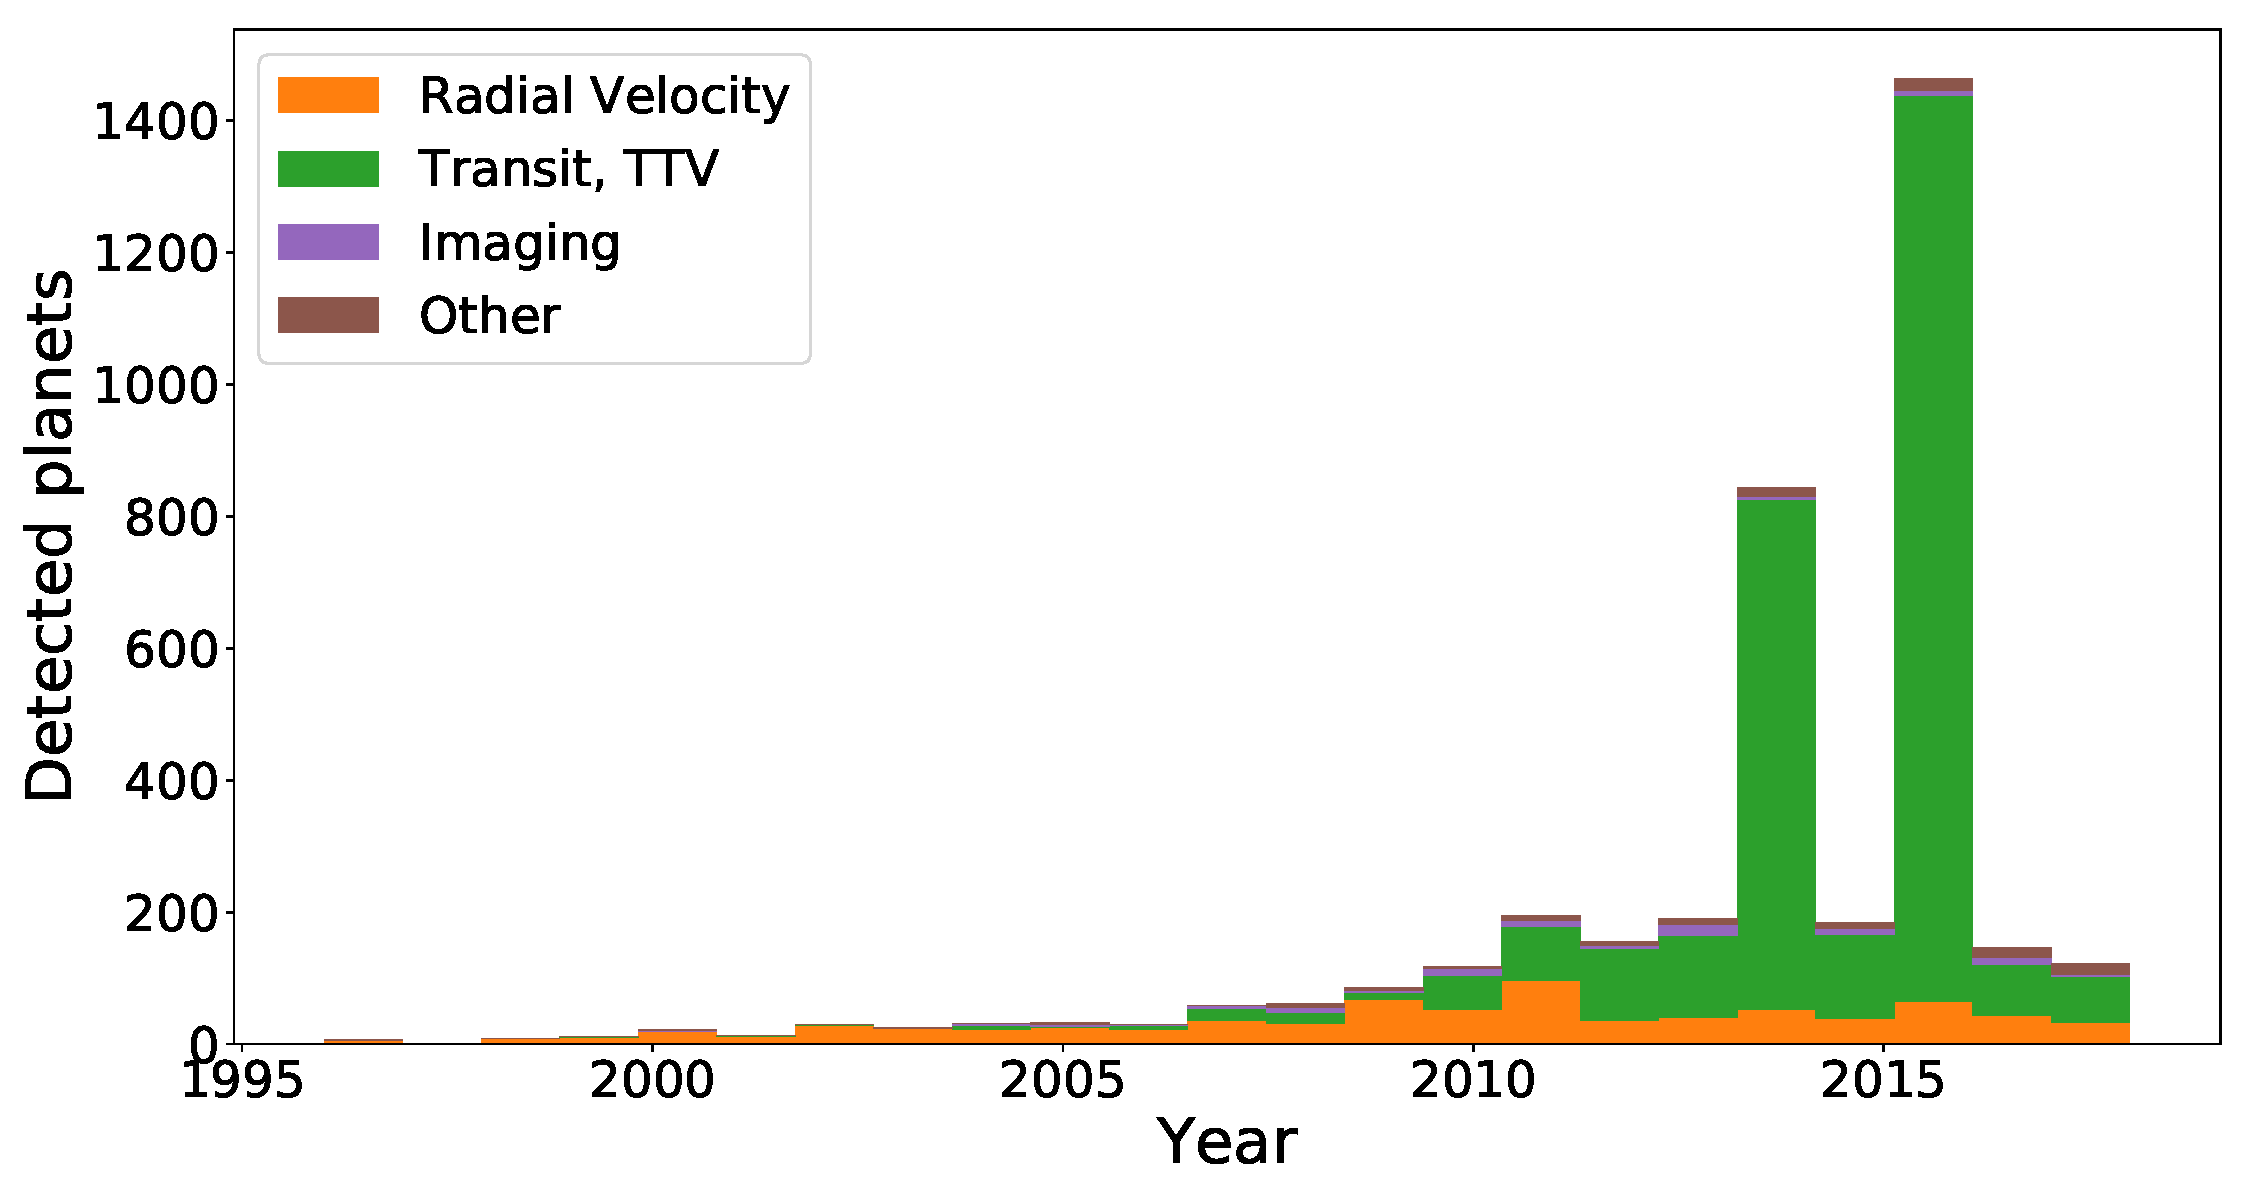
\includegraphics[width=0.7\linewidth]{./figures/introduction/exoplanetEU_year_method.pdf}
    \caption{Number of exoplanet detections per year separated by method (data from \href{http://ww.exoplanet.eu}{exoplanet.eu} October 2018).}
    \label{fig:detection_year_method}
\end{figure}


Details about the various main detection methods are provided in the following sections.

\subsection{Radial Velocimetry}
\label{sub:radial_velocimetry}
This technique measures the radial velocity\footnote{Velocity projected along line of sight.} (RV) of the star by analysing the relative Doppler shift of its spectral lines due to the gravitational interaction with a companion.
As the star and companion orbit around their common centre of mass (barycentre) the spectrum of the star periodically oscillates due to the change in relative motion to the observer as depicted in \fref{fig:rvdiagram-mayor} (left).

The radial velocity variation, directed along the line of sight, is given by

\begin{equation}
\label{eq:rv_equation}
{RV} = \gamma + K [\cos{(\nu(t, P, T_0, e) + \omega)} + e\cos{(\omega)}]
\end{equation}
where $\gamma$ is constant barycentre velocity of the system relative to the Sun\footnote{Earth's barycentre motion is well known and removed.}, \(K\) is the velocity semi-amplitude, \(e\) the eccentricity, and \(\omega\) is the argument of periastron.
The true anomaly \(\nu\), is a function of time \(t\), orbital period \(P\), and the time of periastron passage \(T_0\), and eccentricity.

The velocity amplitude $K$ of a star of mass $\Mstar$ due to a companion with mass $\Mp$ with orbital period $P$, eccentricity $e$, and inclination $i$ is~\citep[e.g.][]{cumming_lick_1999}:

\begin{equation}
    K = {\left(\frac{2\pi G}{P}\right)}^{1/3} \frac{\Mp{} \sin{i}}{{(\Mp{} + \Mstar)}^{2/3}} \frac{1}{\sqrt{1-{e}^{2}}}, \label{eq:k_amplitude}
\end{equation}

where G is the gravitational constant. 

The key exoplanet property determined by the amplitude {RV} technique is the companion mass, relative to the orbital inclination \Mpsini.
As the companion mass is in the numerator of \eref{eq:k_amplitude} the {RV} technique is more sensitive to larger mass planets.
Also since $K \propto P^{-1/3}$ the amplitude is greater for short period close in orbits\footnote{From Kepler's Law ${P}^{2}\propto {a}^{3}$}.

The RV method detected the first exoplanet around a solar-type star {51 Pegasi}~\citep{mayor_jupitermass_1995}, kick-starting the exoplanet discipline.
The first discoveries were surprising as Jupiter mass planets in short period orbits\footnote{\Mpsini=0.47\,\Mjup{} orbiting at 0.05\AU{} for {51 Pegasi}} were unlike anything in our Solar System.
Several exoplanet discoveries followed in quick successions~\citep[e.g.][]{butler_planet_1996, marcy_planetary_1996} with many confirming the existence of the type of planets now referred to as ``hot-Jupiters''~\citep{butler_three_1997, charbonneau_detection_2000}.

The radial velocity amplitudes of the first exoplanets detected were XXX \kmps while 
the radial velocity signal of the Earth in a 1 year orbit around a solar-type star however is 8.9\cmps{}~\citep{figueira_radial_2010}.
Specially constructed spectrographs, such as HARPS~\citep{mayor_setting_2003} along with improve reduction techniques~\citet{lovis_new_2007} spectrographs in the optical pushed this mass detection limit down to the \mps{} level. ESPRESSO~\citep{pepe_espresso_2014, megevand_espresso_2014} is the next generation high precision optical spectrograph aiming to push the detection limits to 10\cmps, to detect an Earth twin.
The gradual decrease in measured mass of exoplanets over time is shown in \fref{fig:exoplaneteuyearmass}. The different symbols indicate the detection method, not necessarily the method used to measure the exoplanet mass.

\begin{figure}
    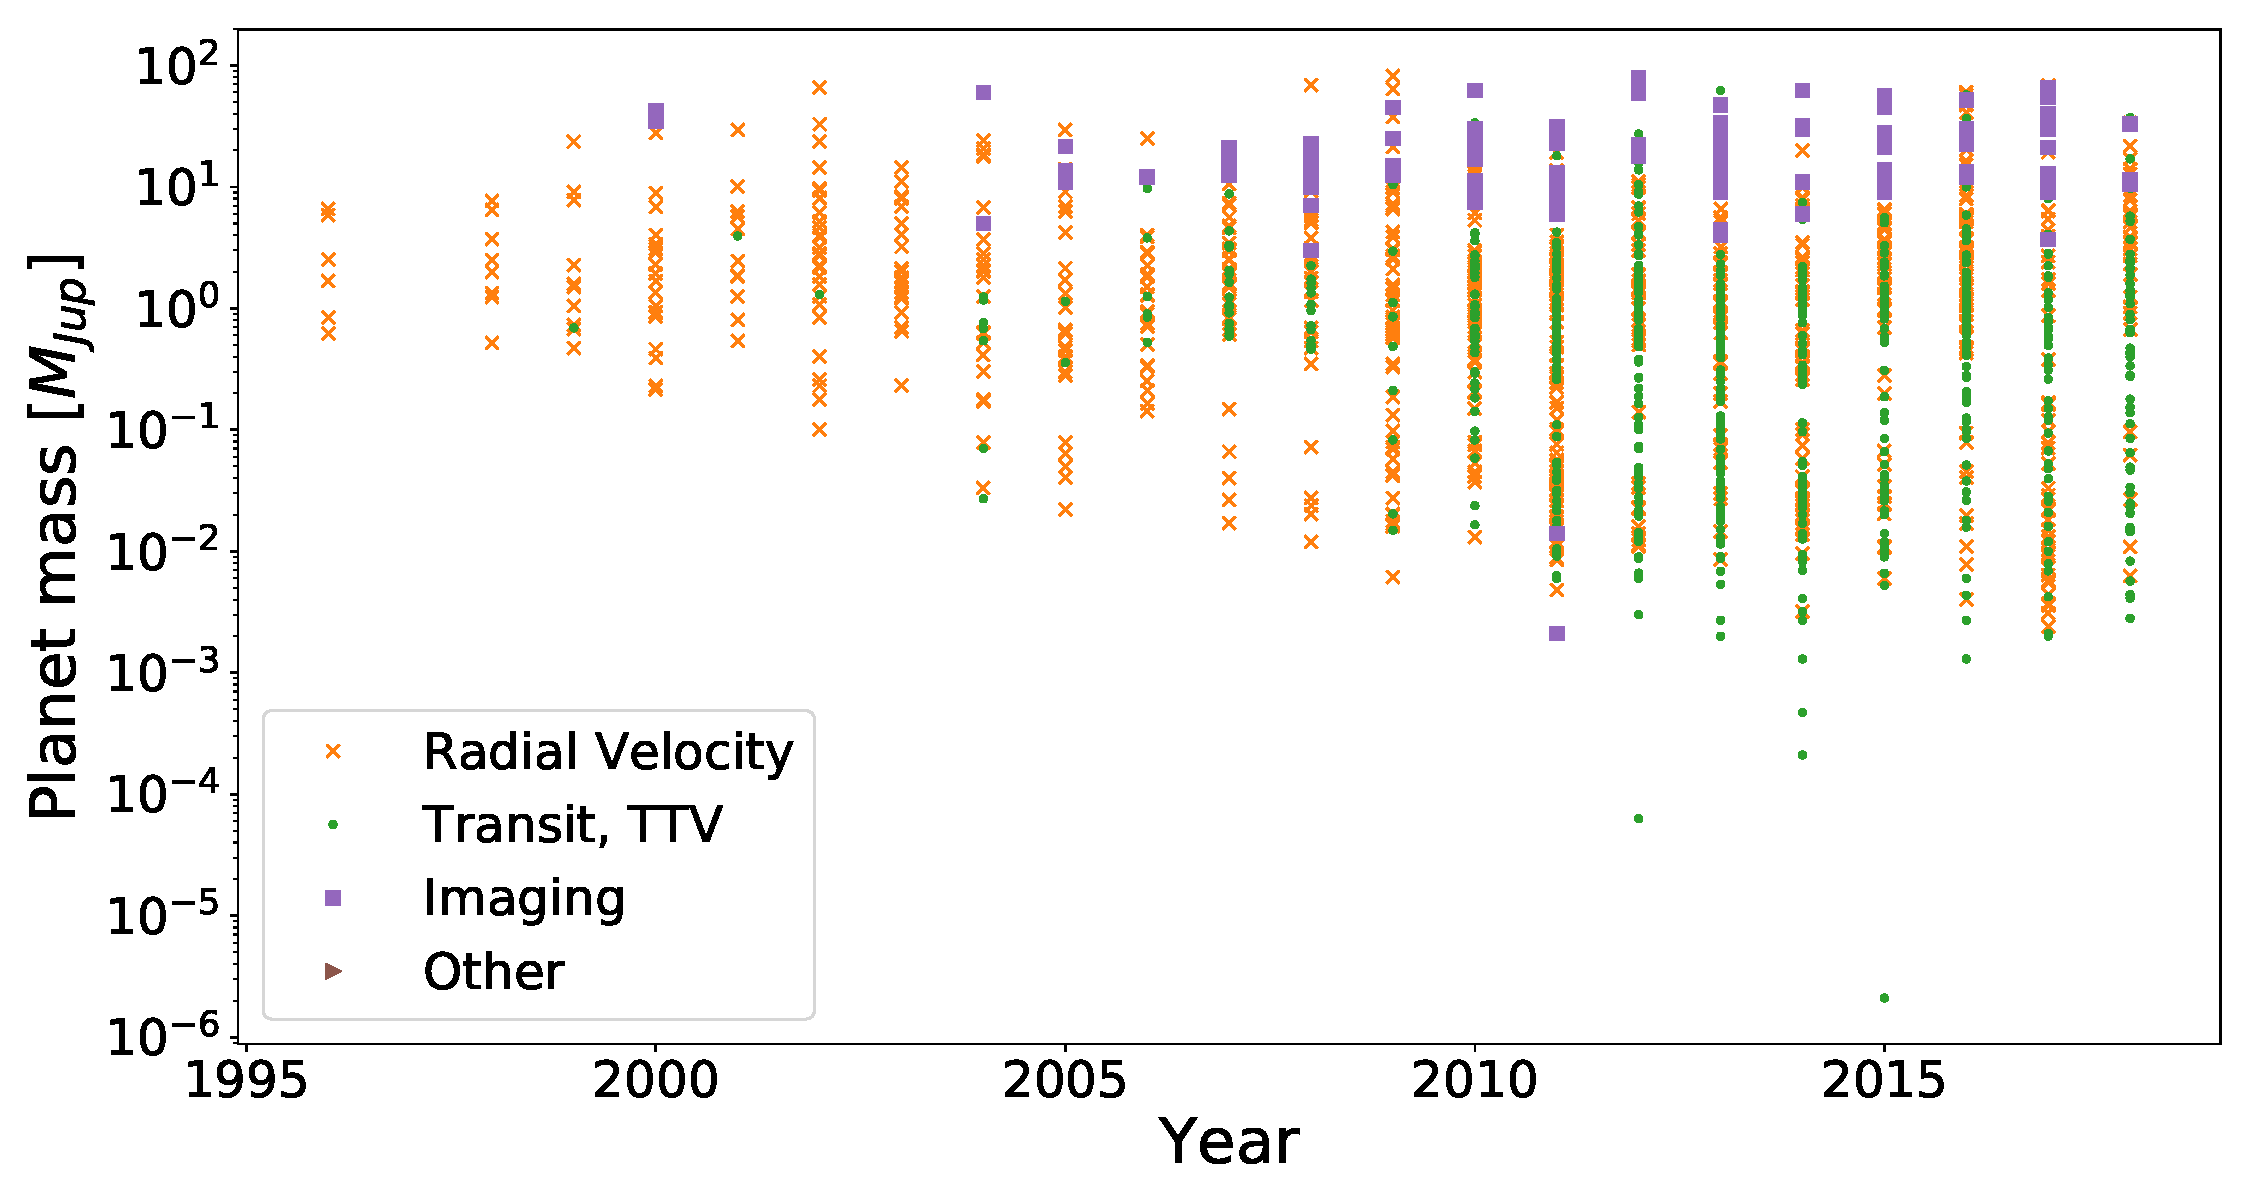
\includegraphics[width=0.5\linewidth]{figures/introduction/exoplanetEU_year_mass.pdf}
    \caption{Exoplanet discovery year verse exoplanet mass. Exoplanets that do not have a measured mass are not shown. Exoplanet mass }
    \label{fig:exoplaneteuyearmass}
\end{figure}

Most {RV} detection has been performed using optical spectrographs.
However, as the amplitude of {RV} signal is inversely proportional to the mass of the star (RV $\propto \Mstar^{-2/3}$), there are dedicated surveys focusing on smaller mass M-dwarf stars\citep[e.g.]{reiners_carmenes_2018}.
M-dwarfs are inherently cooler and thus emit a majority of their stellar output in the near-infrared\reference{cite an M-dwarf paper?}, new dedicated high-resolution \nir{} spectrographs have and are being designed and implemented to meet this demand e.g., {CARMENES}, {NIRPS}, {SPIRou}, {CRIRES+}.

\begin{figure}
    \centering
        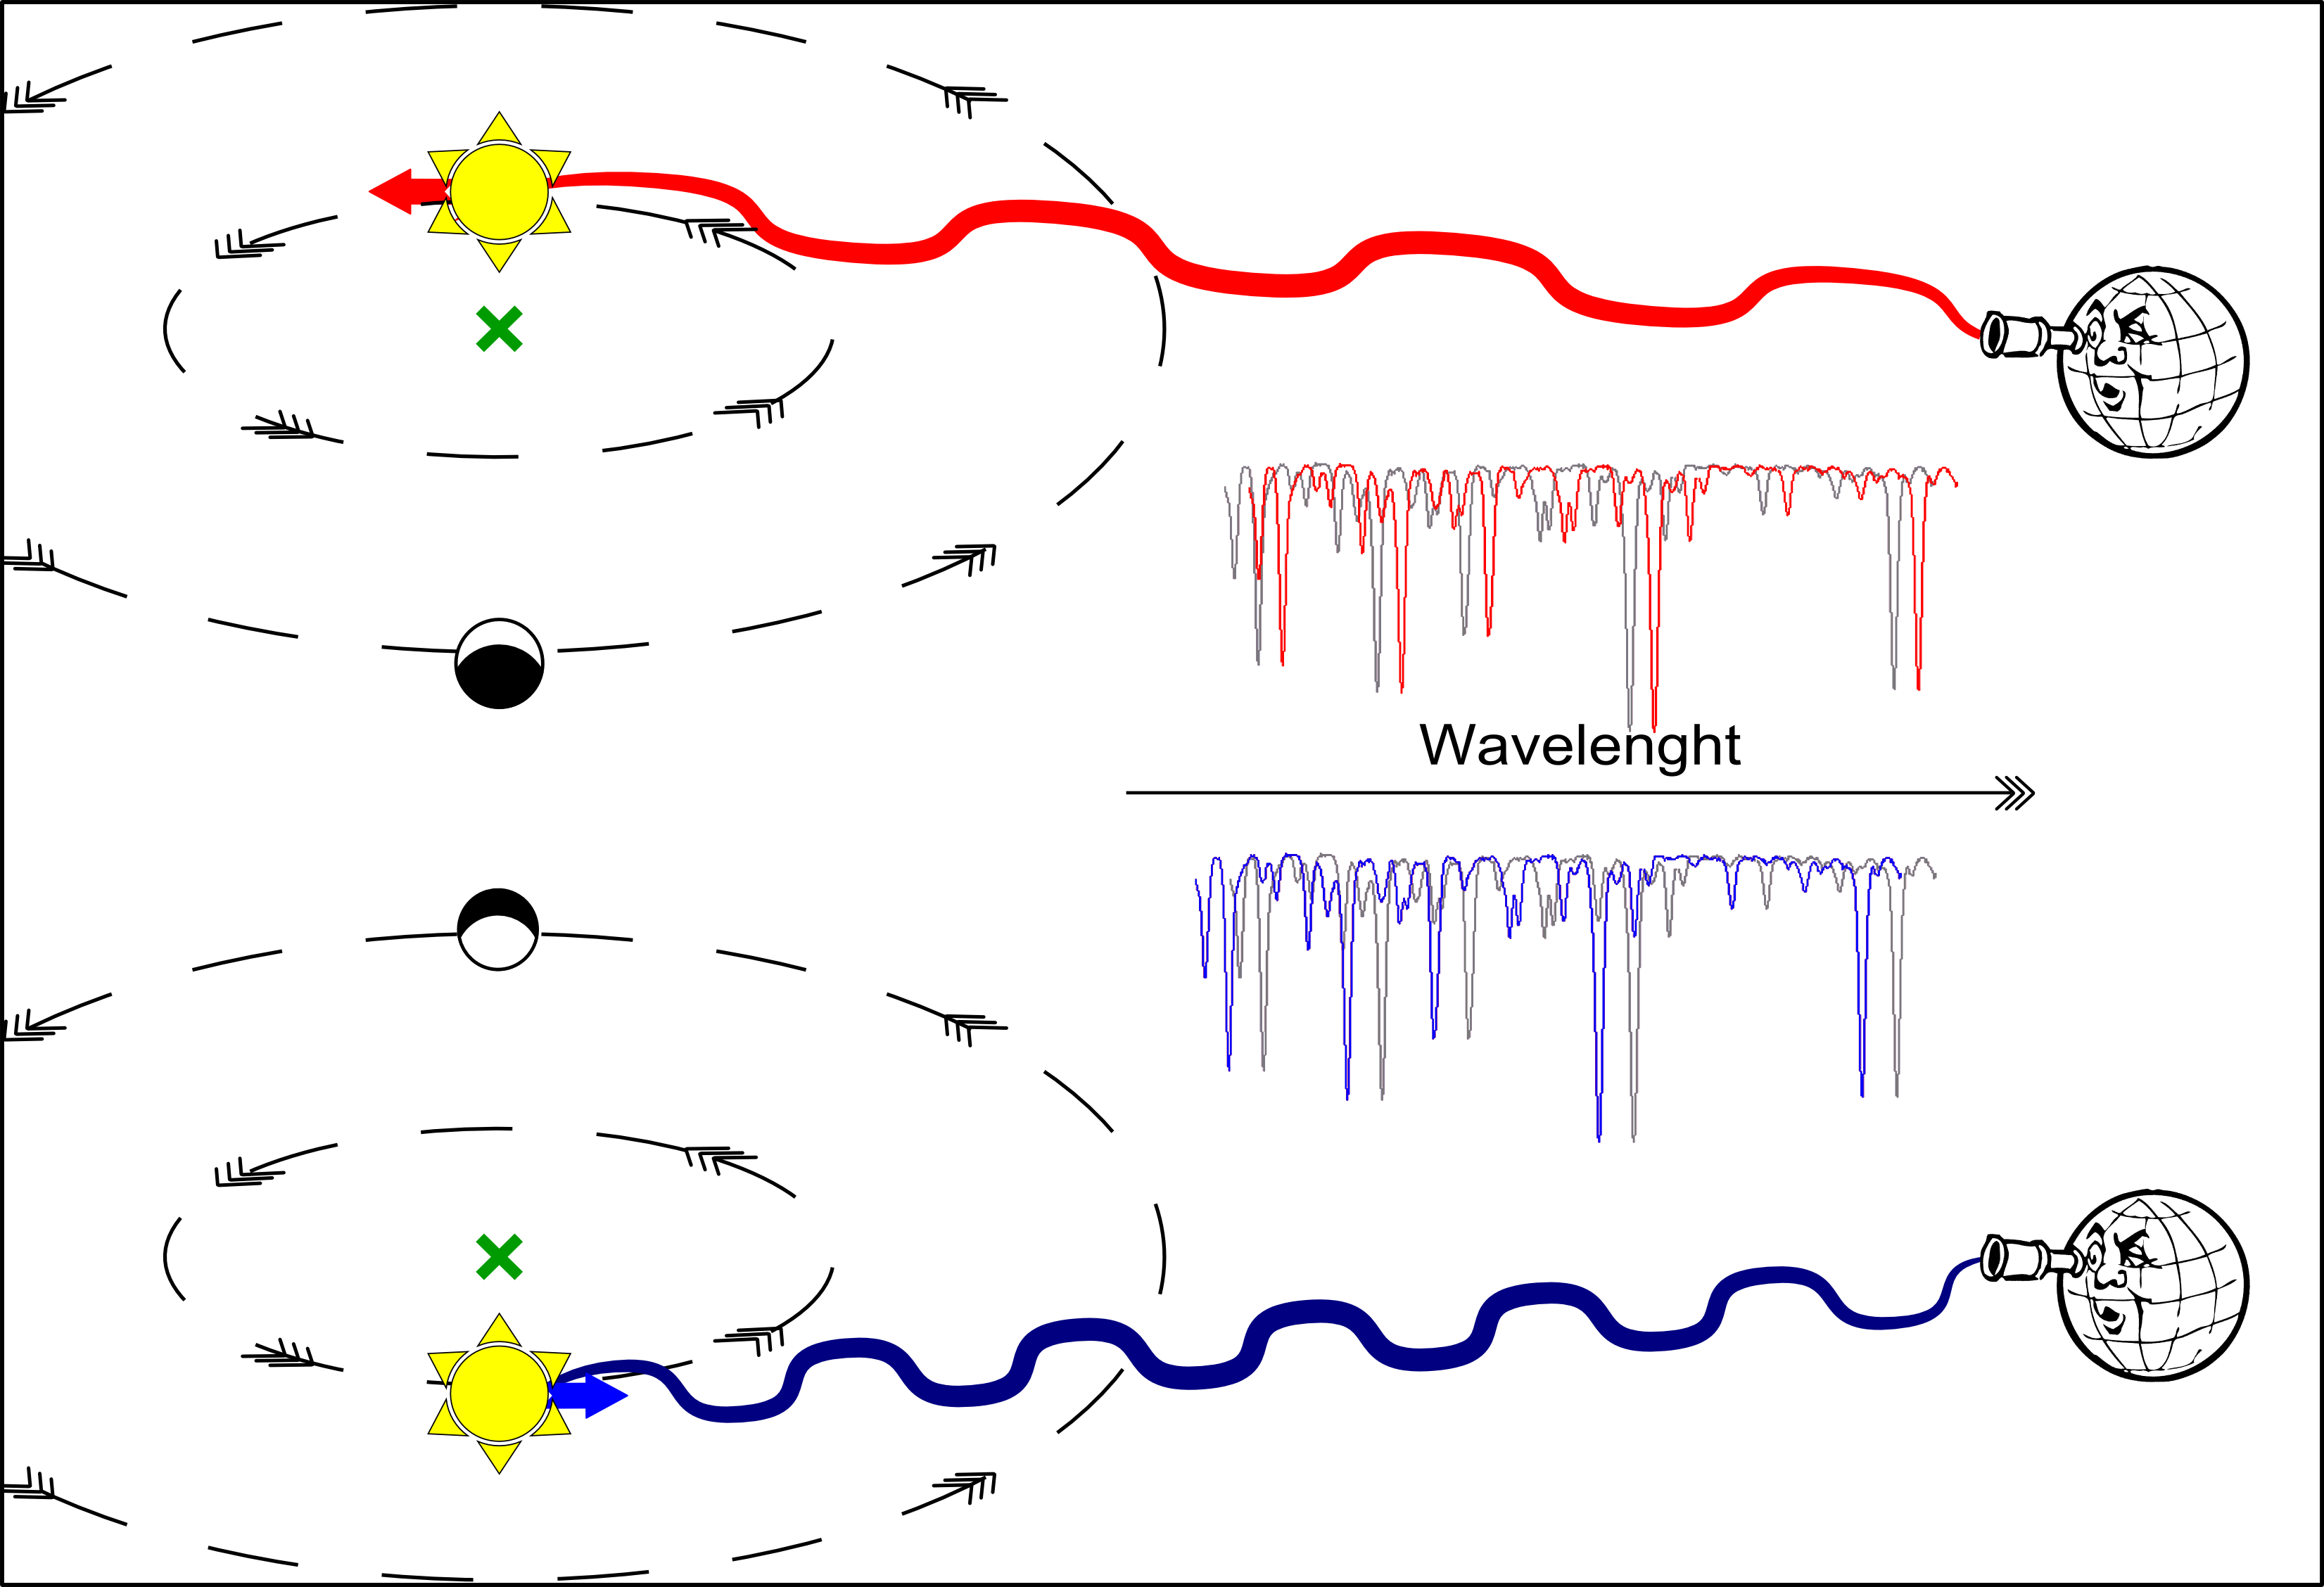
\includegraphics[height=5cm]{./figures/introduction/RV_Diagram}
    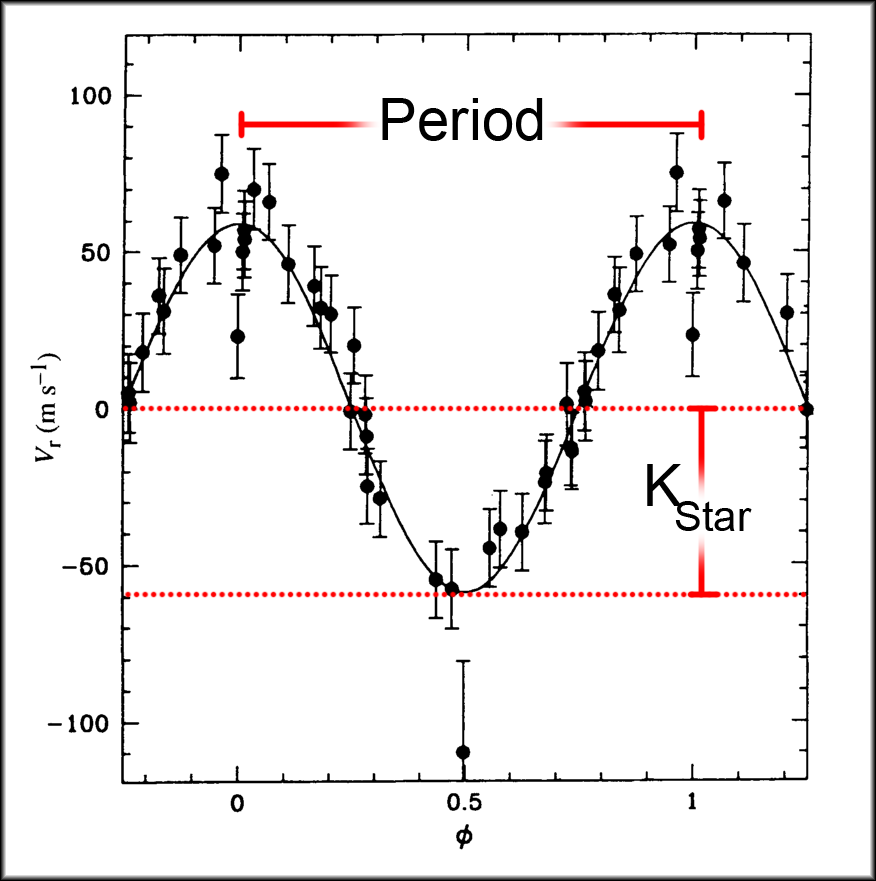
\includegraphics[height=5cm]{./figures/introduction/PhaseFolded_51Pegb_Mayor_et_al_1995}
    \caption{Left: Diagram of {RV} method. Right: {RV} variation for the detection of {51 Pegasi}. Credit:~\citet{mayor_jupitermass_1995}}.
    \label{fig:rvdiagram-mayor}
\end{figure}


\subsection{Transit methods}
\label{sub:transit}
The transit method detects the presence of a exoplanet by observing the periodic dimming of the star due to the passage of the exoplanet between the star and observer, partially blocking the star.
Geometry requires the orbit of the exoplanet needs to be aligned edge-on to the light of sight (low inclinations) for a transit to occur.
The geometric probability, $P$, that a exoplanet transits is estimated by 

\begin{equation}
P \approx \frac{\Rstar}{a (1-{e}^{2})},
\end{equation}

where \(e\) is the eccentricity of the orbit, $\Rstar$ is the star radii and \(a\) is the semi-major axis of the orbit (star-planet distance)~\citep{barnes_effects_2007}.
The probability of transit increases with the size of the star but decreases with distance to the star.

The drop in stellar brightness during the transit allows the measurement of the planet/star radius ratio:

\begin{equation}
    \frac{\Delta L}{L} \sim {\left(\frac{\Rp}{\Rstar}\right)}^{2}
\end{equation}

where \(L\) is the luminosity of the star, \(\Delta L\) is the maximum luminosity variation (transit depth), and \(\Rstar\) and \(\Rp\) are the radius of the star and planet respectively.

The transit method complements {RV} measurements as the inclination, $i$, of the orbit can be determined from the transit.
This removes the {$\sin{i}$} ambiguity found in the \Mpsini{} of {RV} detections so the true mass, $\Mp$, of the exoplanet can be revealed.
The true mass along with the planets radius provides a value for the exoplanets average density\footnote{$\rho \equiv \frac{ \textrm{Mass}}{\textrm{Volume}} = \frac{3}{4\pi}\frac{\Mp}{\Rp^{3}}$}, hinting at the possible composition.

There are several other astrophysical phenomena which can mimic transiting exoplanet signals, created by configurations of two or more stars which may not involve an exoplanet. 
For example a transiting low-mass or white-dwarf star, grazing binary stars, or a transit in a multi-star system~\citep[see e.g.][]{cameron_extrasolar_2012, santerne_contribution_2013}.
Follow-up {RV} observations~\citep[e.g.][]{santerne_radial_2011} are usually required to confirm the planets existence. 
Statistical validation techniques are also possible, such as the PASTIS software~\cite{diaz_pastis_2014}, when follow-up can not be performed.
With {RV} follow-up~\citet{santerne_sophie_2012} found a false positive rate as high as 35\% for short period giant planets, while~\citet{santerne_sophie_2016} found a 54.6\% false positive rate of 129 giant planet with periods less than 400 days.
These sub-sample false positive rates are however higher than the global false positive rate of 9.4\%~\citep{fressin_false_2013}/ 11.3\%~\citep{santerne_contribution_2013} found for Kepler.
Some of the currently known exoplanet systems with the smallest radii and lightest mass have been detected through transit and later confirmed with high-precision {RV} follow-up~\citep[e.g.][]{queloz_corot7_2009, pepe_earthsized_2013, lopez-morales_kepler21b_2016, ment_second_2018}.

The transit of a single planet can not directly determine the planetary mass.
However, in multiple planet systems, the masses and sometimes the presence of other planets in the system can be determined from perturbations in the transit time and duration~\citep[e.g.][]{holman_use_2005, holman_kepler9_2010}.
A large number of systems have been detected that show transit timing variations (TTV) and transit duration variations (TDV)~\citep[e.g.][]{holczer_transit_2016} due to the gravitational interaction between planets.
The statistical validity of multi-transiting planets is also higher than single planets as probability of multiple false positive is lower than having multiple planets in the system~\citep{lissauer_almost_2012}, making them easier to validate.

The presence of star spots on the surface of a star can be observed during transit.
A star spot is a dark region on the stellar surface due to magnetic fields, which decrease the luminosity slightly. Examples of spots can be seen in the middle of Sun from an image of the 2012 transit of Venus in \fref{fig:transit_venus_transit_alignment}(left). It shows several dark Sun spots along side Venus, although Venus did not cross them. Unlike for other stars, Sun spots can be spatially resolved.
If an exoplanet passes in front of a spot, the luminosity decrease from the spot is temporarily hidden and a small bump occurs in the transit shape.
The presence of spots in successive transits (see \fref{fig:fig:transit_venus_transit_alignment}(right)) can indicate the alignment of the stellar rotation to the planet orbital plane~\citep{sanchis-ojeda_starspots_2013}. In this simulation an orbit aligned with the stellar rotation and the transit crosses the spot in four successive orbits. In a misaligned case a spot would only be observed in one transit.

\begin{figure}
    \centering
    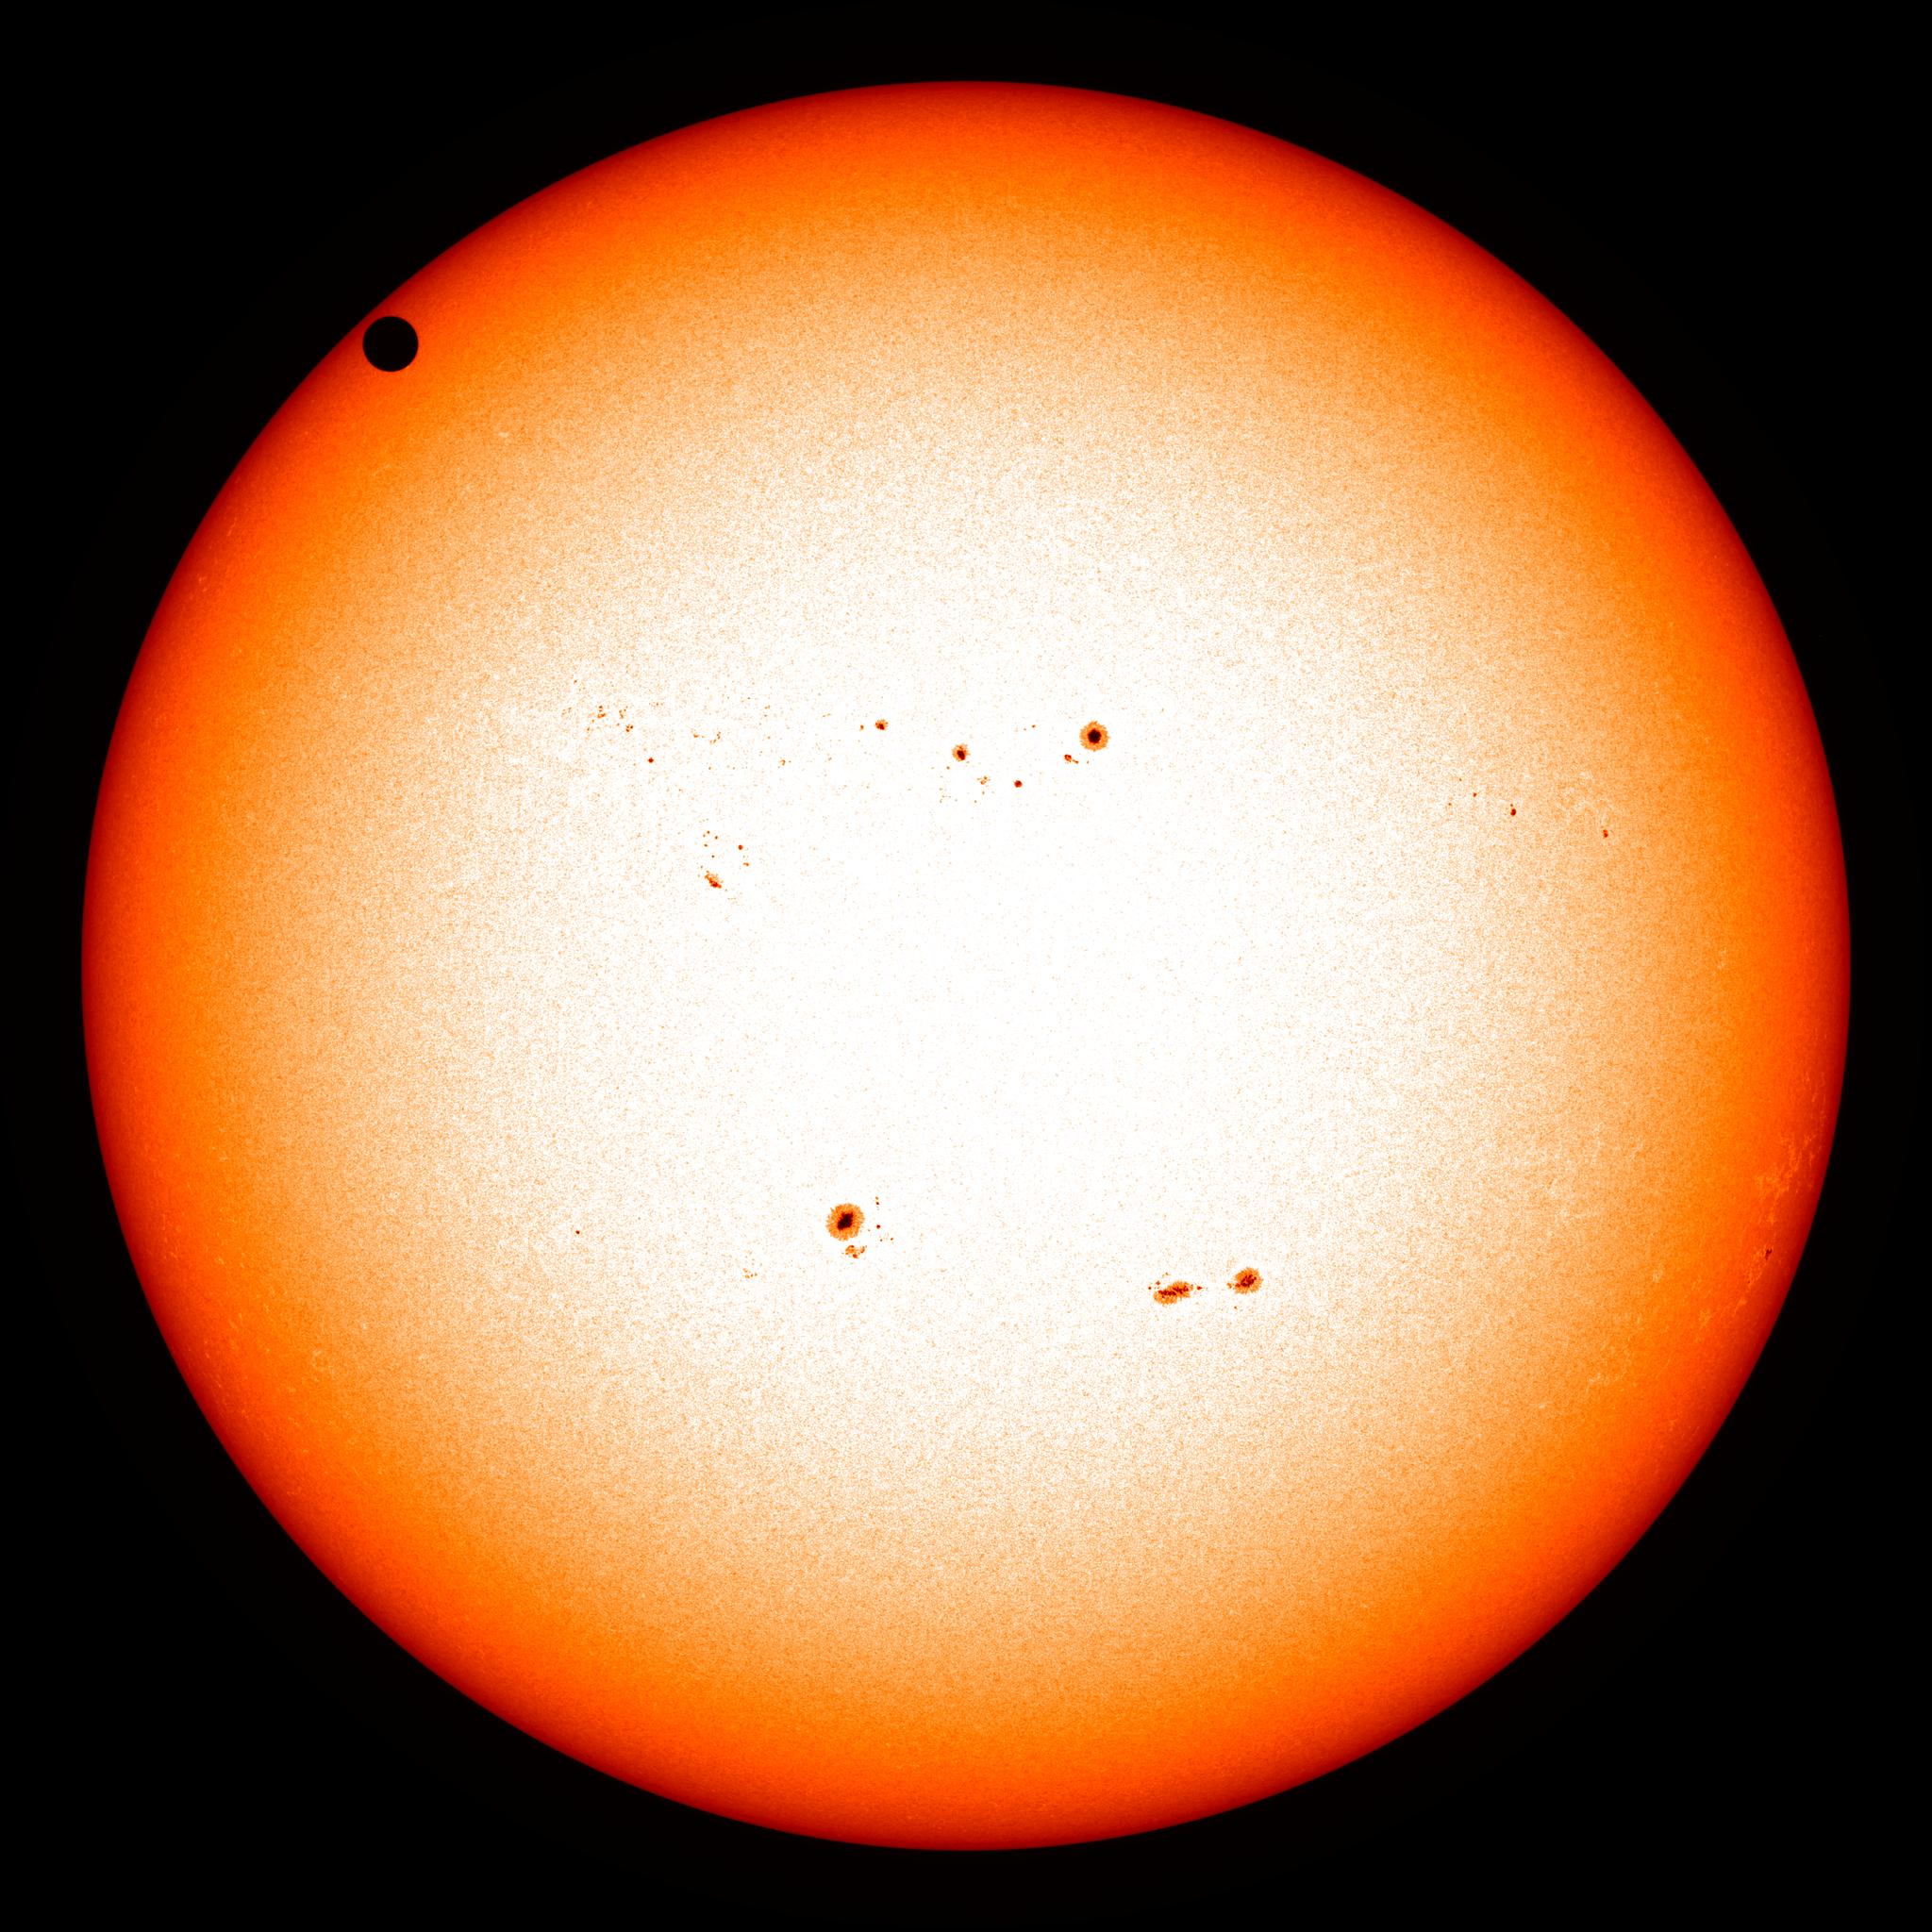
\includegraphics[height=5cm]{./figures/introduction/SDO_2012_Venus_Transit.jpg}
    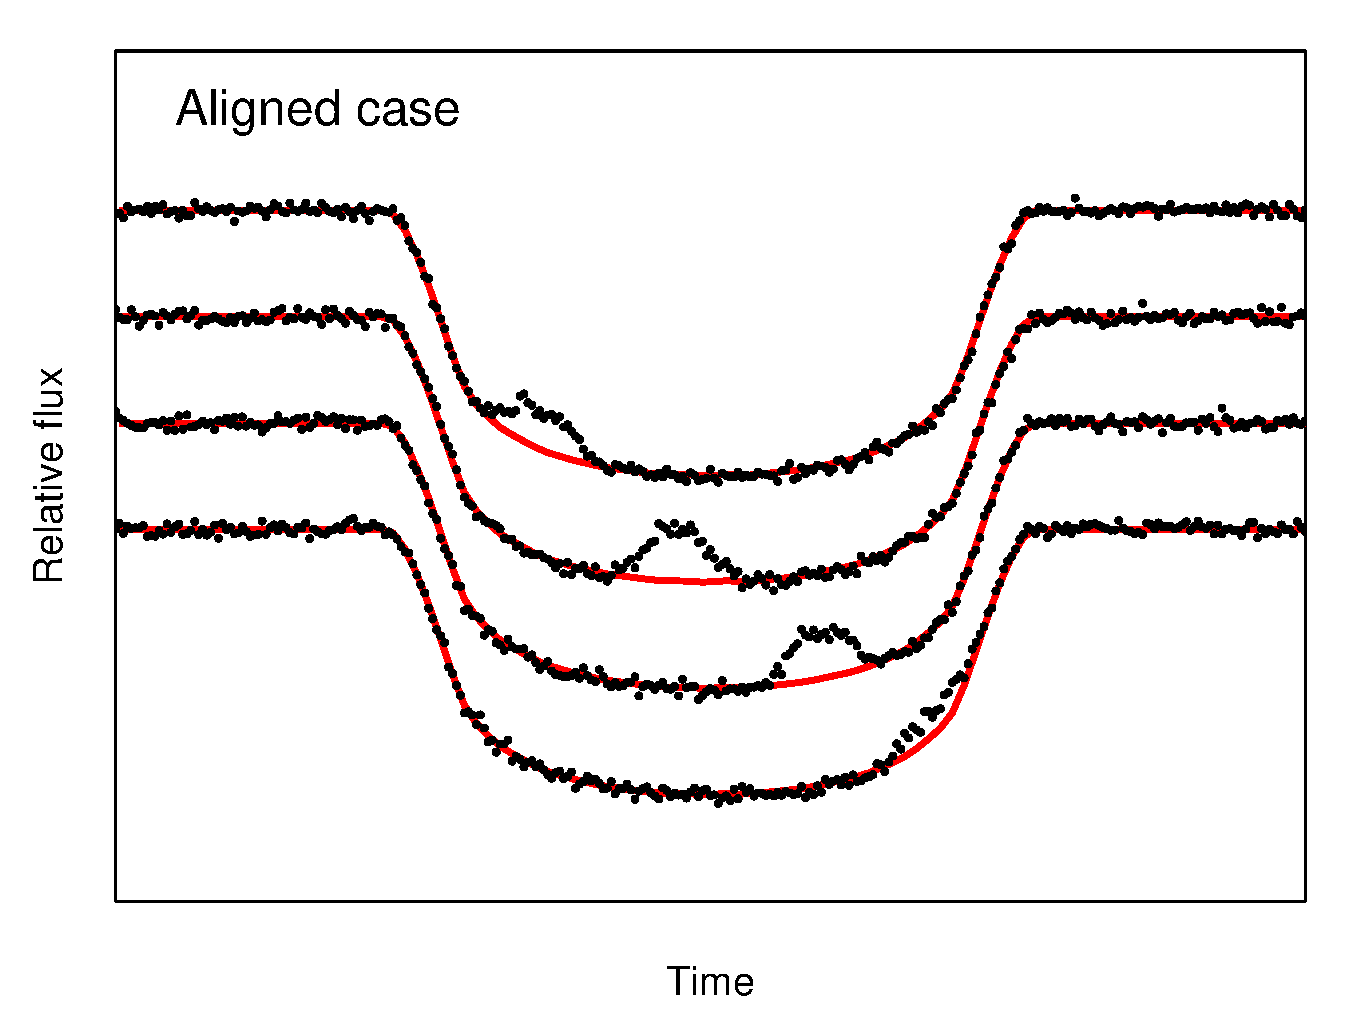
\includegraphics[height=5cm]{figures/introduction/sanchisojedafig1-crop.pdf}
    \caption{Left: Image from the 2012 transit of Venus obtained from Solar Dynamics Observatory satellite. Venus is the dark circle in the top left of the Sun. Limb darkening is observed as the change in colour/brightness from white to red near the edge. Several sunspots are also observed on the surface of the Sun.
    Credit: NASA/SDO, HMIR. Right: Simulation of 4 successive transits crossing a star spot with the orbit aligned with the stellar rotation. The stellar rotation is 1/10 the orbital period. Adpated from~\citet[][Figure~1]{sanchis-ojeda_starspots_2013}.}
    \label{fig:transit_venus_transit_alignment}
\end{figure}


The vast majority of transit detections have come from Kepler~\citep{borucki_characteristics_2011}, which focused on a small patch of sky (0.25\%) for four years continuously.
However, {CoRoT}~\citet{barge_transiting_2008} and ground-based surveys are also WASP~\citep{pollacco_wasp_2006}, OGLE~\citep{udalski_optical_2002}, TreS~\citep{alonso_tres1_2004} have also had successful transit detections.

Following in Kepler's footsteps the next generation transit hunter {TESS}~\citep{ricker_transiting_2015} has already announced discoveries of new transiting planets only months after launch~\citep{vanderspek_tess_2018, gandolfi_tess_2018, huang_tess_2018}.
It will eventually cover more than 90\% of the sky with an impressive planetary yield expected of $\sim$10\,000 exoplanets, with around 3500 the size of Neptune or smaller~\citep{barclay_revised_2018, huang_expected_2018}.
However, the observation coverage is not uniform, with the majority of the ecliptic plane receiving only one month of observations, limiting the detection sensitivity to short period transiting planets. The ecliptic poles will receive almost one year continuous observation.


\subsection{Direct Imaging}
\label{sub:direct_detection}
The direct imaging technique involves directly imaging an exoplanet in orbit around a star.
The first planets directly imaged were {2MASSWJ~1207334--393254~b} using adaptive optics with NACO on the LVLT\citep{chauvin_giant_2004}, three planets around HR\,8799 using angular differential imaging on the Keck and Gemini telescopes~\citep{marois_direct_2008}, and {Fomalhaut~b} using chronography on the HST~\citep{kalas_optical_2008}.
As an example the direct image of {HR\,8799} is shown in \fref{fig:directimaging}, where a fourth planet was revealed~\citep{marois_images_2010}.

Direct imaging requires resolving the angular separation between the star and planet and is best suited to detect giant planets in wide orbits (>10\AU{}) around nearby stars. This is shown by the clustering of direct image detections shown in \fref{fig:exoplaneteuyearmass}.
Extremely young giants observed in the infrared are favoured as they have higher thermal emission (while they are still cooling) and larger surface area resulting in a higher contrast ratio to the host.\todo{Reference this}


\begin{figure}
    \centering
    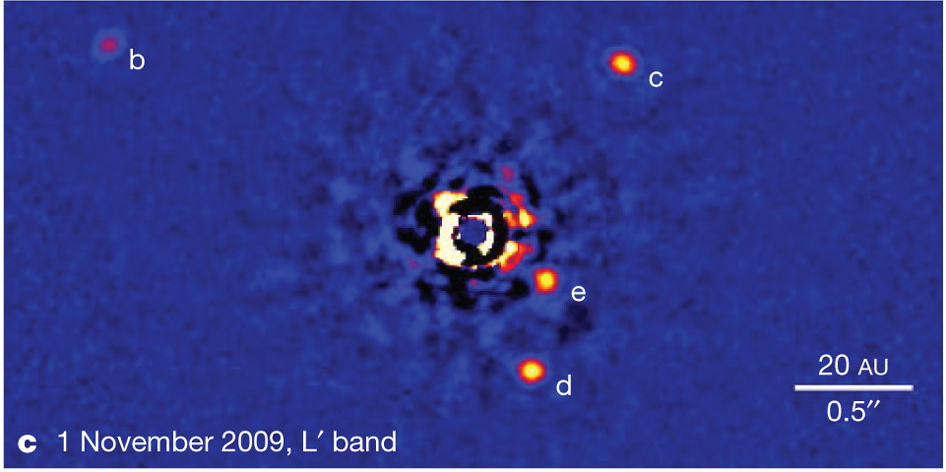
\includegraphics[width=0.5\linewidth]{./figures/introduction/DirectImaging_HR8799_MaroisEtAl2010}
    \caption{Direct detection of four exoplanets around HR\,8799~\citep{marois_images_2010}.}
    \label{fig:directimaging}
\end{figure}

High-contrast adaptive optics instruments, such as SPHERE@VLT~\citet{beuzit_sphere_2008} and GPI~\citep{macintosh_gemini_2008}, are being used with several different techniques to observed targets closer to the star and with smaller contrasts, usually involving blocking or cancelling out the light from the star while keeping the planet \citep[e.g.][]{marois_direct_2005, mawet_annular_2005, schmid_zimpol_2005, sirbu_prospects_2017, sirbu_techniques_2017, wang_observing_2017}.
Ground based direct imaging requires adaptive optics to reduce the turbulence induced by the atmosphere, increasing the angular resolution down to the telescope diffraction limit. 

Along with exoplanets direct imaging is also used to observe circumstellar and protoplanetary disks, and even image planets during formation \citep[e.g.][]{sallum_accreting_2015}.
Combining direct images from different photometric bands can allow for the creation of low-resolution exoplanet spectra \citep[e.g.][]{kuzuhara_direct_2013, zurlo_new_2015}.


\subsection{Astrometry}
\label{sub:astrometry}
Astrometry measures the precise position of the stars on the plane of the sky.
The motion of a star with an exoplanet about its centre of mass can be observed in the periodic oscillating of position from its proper motion in the sky.

For a circular orbit the angle of the semi-major axis of the apparent orbital ellipse, the amplitude of the astrometric signature ($\theta$), is given by

\begin{equation} 
\theta = \frac{M_{p}}{M_{star} + M_{p}} \frac{a}{d}
\end{equation}

where, $\Mp$ and $\Mstar$ are the planet and stellar mass, $a$ is the semi-major axis (in \AU) and $d$ is the distance from the observer to the system (in parsec)~\citep{perryman_exoplanet_2011}.

This shows that the astrometric signal is proportional to the companion/star mass ratio and to the orbital radius, $a$.
The amplitude also decreases inversely with distance, as the angles become smaller.
This is unlike the {RV} and transit methods for which the amplitude is not affected by distance.
Astrometry is complementary to the {RV} method as it measures the orbital motion perpendicularly to the line of sight, allowing the three-dimensional orbit to be determined.

A modelled astrometric signal is shown in \fref{fig:astrometry_perryman}, for a star at a distance of 50\pc, with a proper motion of 50\masperyr{}, and orbited by a planet of $\Mp = 15$\,\Mjup{}, $e = 0.2$, and $a = 0.6$\AU~\citep{perryman_extrasolar_2000}.
The straight dashed line shows the path of the system's barycentric motion viewed from the Solar System barycentre.
The dotted line shows the effect of parallax (the Earth's orbital motion around the Sun, with a period of 1 year).
The solid line shows the apparent motion of the star as a result of the planet, the additional perturbation being magnified by $\times 30$ for visibility.

Although astrometry has detected many binary stars~\citep[e.g.][]{gontcharov_new_2000} and found several brown-dwarf companions~\citep[e.g.][]{sahlmann_search_2011}, the exoplanet discovery's are few.
A 1.5\,\Mjup{} mass planet in a roughly 1000 day orbit around {HD\,176051} was reported by~\citet{muterspaugh_phases_2010}, and recently the astrometric perturbation of a known planet, {Beta Pictoris~b}, was performed utilizing measurements from {GAIA}~\citep{gaiacollaboration_gaia_2016} and {HIPPARCOS}~\citep{esa_hipparcos_1997} to determine a mass of 11\,\Mjup~\citep{snellen_mass_2018}.

The predicted astrometric variations for an exoplanet are at the level of sub-milliarcsecond are not achievable from the ground due to atmospheric turbulence.
The most precise astrometric measurements, come from spacecraft, and are currently being performed with GAIA, recently providing astrometric parameters 1332~million sources~\citep{collaboration_gaia_2018} and reaching an precision of 0.04\,mas for the brightest stars (<14 magnitude).
Simulations predict that more than 21\,000 large mass planets (1--15\,\Mjup) in long-period orbits should be discovered during the 5 year nominal GAIA mission~\citep{perryman_astrometric_2014}. 

\begin{figure}
    \centering
    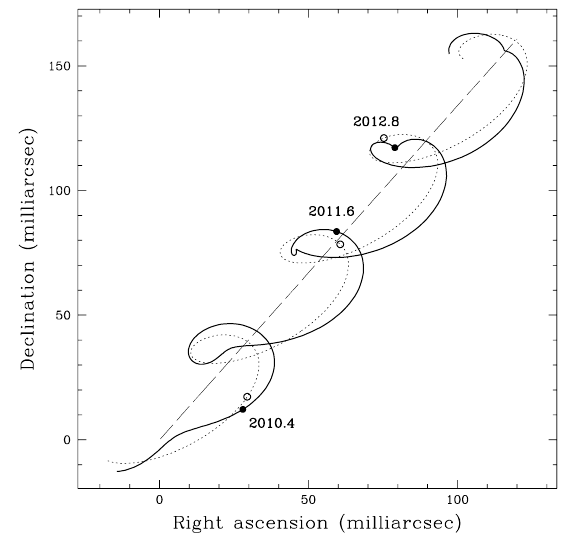
\includegraphics[width=0.5\linewidth]{./figures/introduction/Astrometry_Perryman2000.png}
    \caption{The modelled path on the sky from~\citet{perryman_extrasolar_2000}. Showing a star at a distance of 50\pc, with a proper motion of 50\masperyr{}, 
        and orbited by a planet of $\Mp$ = 15\,\Mjup{}, $e$ = 0.2, and $a$ = 0.6\AU{}.
        The straight dashed line shows the path of the system's barycentric motion viewed from the Solar System barycentre. 
        The dotted line shows the effect of parallax (the Earth's orbital motion around the Sun, with a period of 1 year).
       The solid line shows the apparent motion of the star as a result of the planet, the additional perturbation being magnified by $\times 30$ for visibility.
    }
    \label{fig:astrometry_perryman}
\end{figure}


\subsection{Microlensing}
\label{sub:microlensing}
Microlensing is an astronomical effect predicted by Einstein's General Theory of Relativity.
The mass of an object bends space-time which causes light to be visibly deflected around large mass objects.
As a star passes between Earth and a distant star it acts like a lens, bending and magnifying the light from the background star.
The gravitation of a planet orbiting the lens star (if it exists) creates a distortion in the lens, leading to small caustics, deviations in the single lens microlensing light curve.

An example is shown in \fref{fig:microlensing_example} where a lensing magnification of up to $\times3$ is observed for {OGLE2005-BLG-390}~\citep{beaulieu_discovery_2006}.
On the falling edge of the lensing event (and inset top right) there is a bump due to the presence of a 5.5\,\Mjup{} companion.

The difficulties of microlensing is that they require the chance alignment between Earth, a nearby lens star, and a distance source star, which is unrepeatable.
Some caustics are often difficult to fit and yield degenerate results, making characterization of the planet difficult.
Follow-up measurements of a handful of have been performed~\citep[e.g.][]{kubas_frozen_2012, batista_confirmation_2015, santerne_spectroscopic_2016} to break degeneracies. 
However, follow-up can be difficult as microlensing is sensitive to distant host stars, which are outside the ability of current spectrographs.
It is also sensitive to planets with a wider orbital separation compared to transits and {RV}.
Currently there are 82 planets in 79 systems detected by microlensing, as listed in the \href{https:\\www.exoplanet.eu}{exoplanet.eu} database.

Microlensing events are detected and monitored using dedicated global telescope networks such as {OGLE}, {MOA}, {microFUN} and {PLANET}.
They focus their viewing towards the galactic bulge where there are more stars and a higher chance for microlensing events to occur.

The precise stellar proper motions from the GAIA mission are being used to predict possible future alignments what could produce microlensing events~\citep{kluter_prediction_2018} 

\begin{figure}
    \centering
    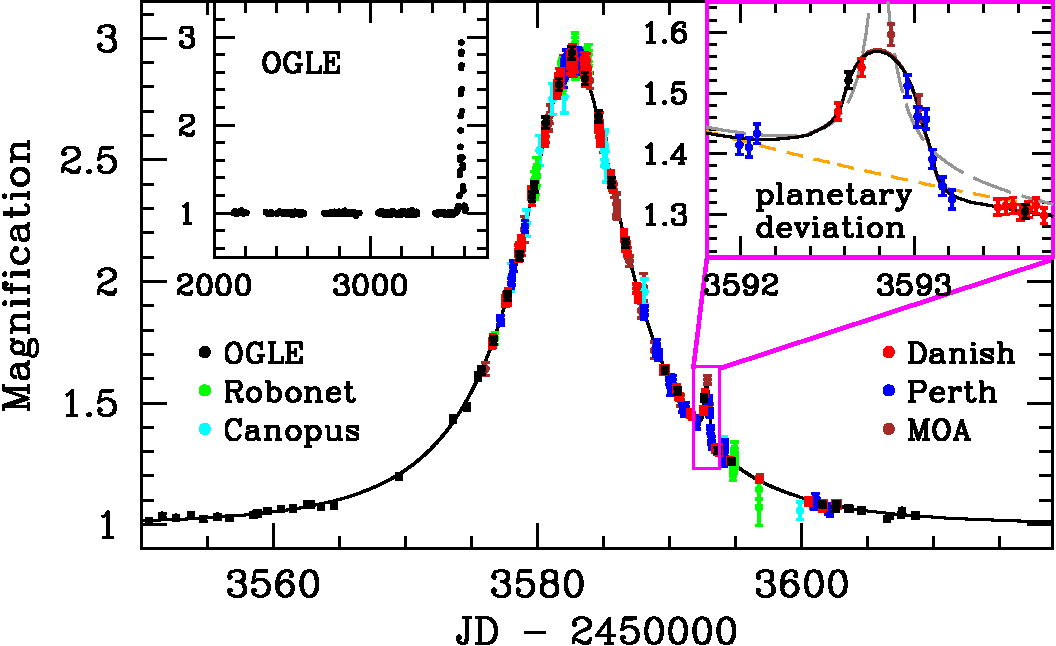
\includegraphics[width=0.5\linewidth]{./figures/introduction/Microlensing_OGLE2005-BLG-390.pdf}
    \caption{Microlensing magnification of OGLE2005-BLG-390 from~\citep{beaulieu_discovery_2006}.
    The presence of the 5.5\,\Mjup{} planet causes the small bump shown in the upper right inset plot.}
    \label{fig:microlensing_example}
\end{figure}


\subsection{Pulsar timing}
\label{sub:pulsar_timing}
Pulsars are rapidly rotating neutron stars or white dwarfs formed after the death of a giant star, that radiate an intense electromagnetic beam.
The timing variations of the millisecond pulsar\footnote{Rotating at 9\,650 revolutions per minute} {PSR1257+12} led to the first extrasolar planet detection~\citet{wolszczan_planetary_1992}.
The are two models of planet formation around pulsars: either they formed before the supernova explosion and survived, or they formed after, from the remnants of the supernova explosion~\citep{Starovoit_existence_2017}
There is still a rarity of <10 pulsars with orbiting planets known.


\section{Detecting atmospheres}
To help characterize an exoplanet, a detection of its atmosphere can provide useful information. After the detection of exoplanets and the measurement of bulk properties, the next goal is detecting the atmosphere.  are being developed to available to this can give rise to the composition of the atmosphere, density, thickness
To enhance the characterization of exoplanets

Several techniques that are showing interesting results are detailed below phase vriation, transmission spectroscopy and direct detection.

\subsection{Secondary transit and phase variations}

Secondary transit and phase variations are an extension of the transit method, requiring higher precision to detect the refelction and thermal emmision of the exoplanet. The star with orbiting exoplanet is photometrically monitored over the whole orbit. An example diagram of phase variation is shown in \fref{fig:transits_and_occultations} as the solid blck line. Starting with the primary transit at the bottom, in which the planet is blocking the star. The light measured during transit is not only the unblocked light from the star but also the thermal emission from the night side of the planet. Immediately before and after transit there will be the full flux from the star plus the emission from the night side of the planet. As the planet orbits around the star the fraction of the day side of the planet visible will change up to maximum when the full day side of the planet is visible. If the alignment is correct the planet will pass behind the star causing an occultation. At this point the only light received is from the star alone.

The depth of the occultation is a measure of the flux from the day side of the planet which can indicate the atmospheric reflection and thermal emission of the planets atmosphere. 
Continuing on in the orbit the phase of combined star + planet again reduces as more of the night side faces Earth.

\fref{fig:stevensonphasecurve2014} shows a real example of the phase folded light curve measured with the HST over several orbits~\citep{stevenson_thermal_2014}.

The primary transit is shown inset with a depth of 2.5\%. The phase variation out of primary transit reaches a maximum of around 0.04\%. The occultation occurs at a phase of 0.5 but it is clearly noticeable that the peak of brightness in the light phase curve slightly leads the occultation. This indicates that the brightest point on the planet is not directly towards the planet. and there is heat redistribution.

thermal profile/phase of hot spot. 


\begin{figure}
    \centering
    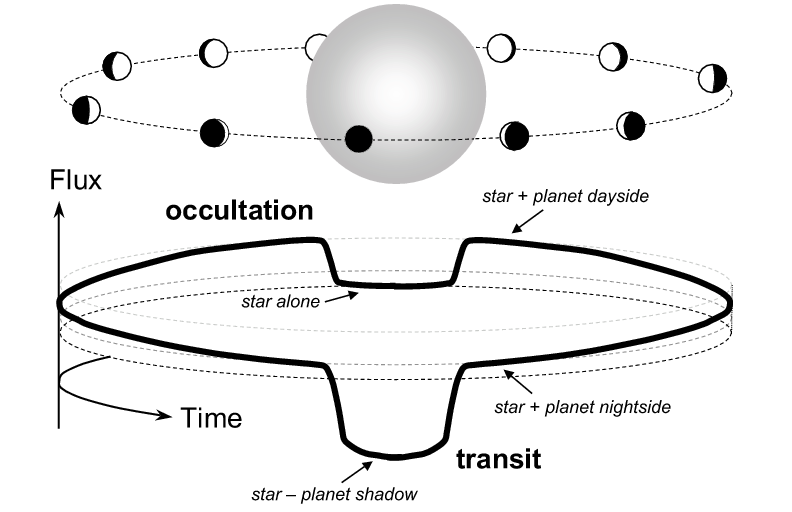
\includegraphics[width=0.6\linewidth]{./figures/introduction/circular_diagram.png}
    \caption{Illustration of transits and occultations.
        Only the combined flux of the star and planet is observed.
        During a transit, the flux drops because the planet blocks a fraction of the starlight.
        Then the flux rises as the planet’s dayside comes into view.
        The flux drops again when the planet is occulted by the star. Credit~\citet{winn_transits_2010}}
    \label{fig:transits_and_occultations}
\end{figure}
\todo{caption directly from source- maybe adapt??}


\begin{figure}
    \centering
    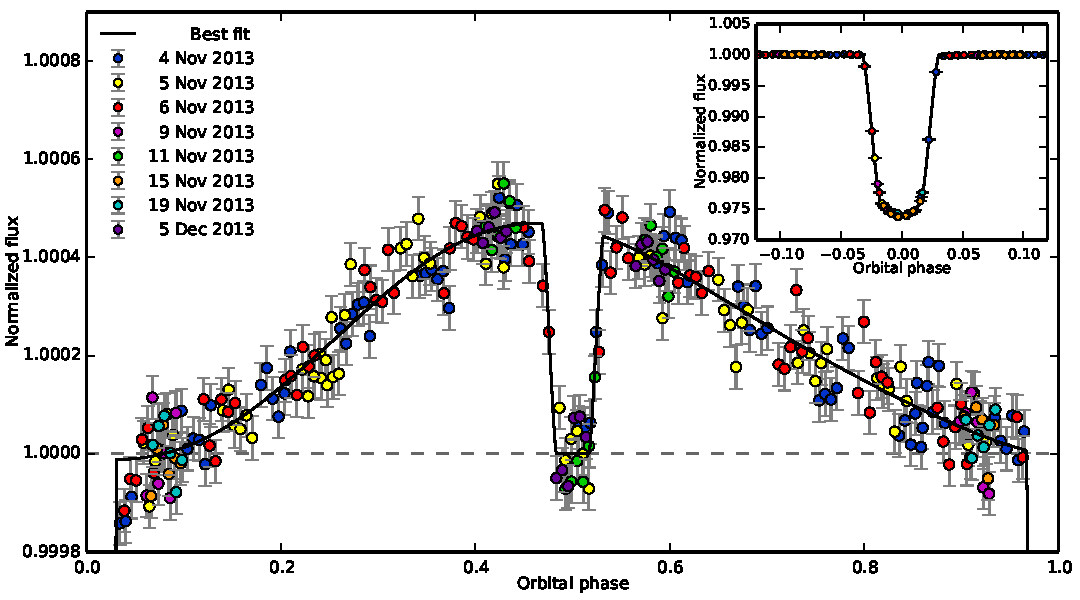
\includegraphics[width=0.6\linewidth]{figures/introduction/stevenson_phasecurve2014}
    \caption{Measured phase variation of XXX with HST. The peak of brightness occurs before the secondary transit, indicating heat distribution of the  \cite{stevenson_thermal_2014}}
    \label{fig:stevensonphasecurve2014}
\end{figure}



\subsection{Transmission spectroscopy}
radius changes with wavelength, extra absorption during transit can give molecular composition.

snellen  et al


Transit and occulations~\citet{winn_transits_2010}

Detection of winds


\subsection{Phase variations}



\subsection{High resolution spectroscopy}
Snellen  Brogi, de Kok

Cross correlation mle  \citet{piskorz_evidence_2016}



\subsection{Stellar and planetary formation}

Brown dwarfs

\subsection{Exoplanet distribution} 4 different groups

\fref{}


\begin{figure}
    \centering
    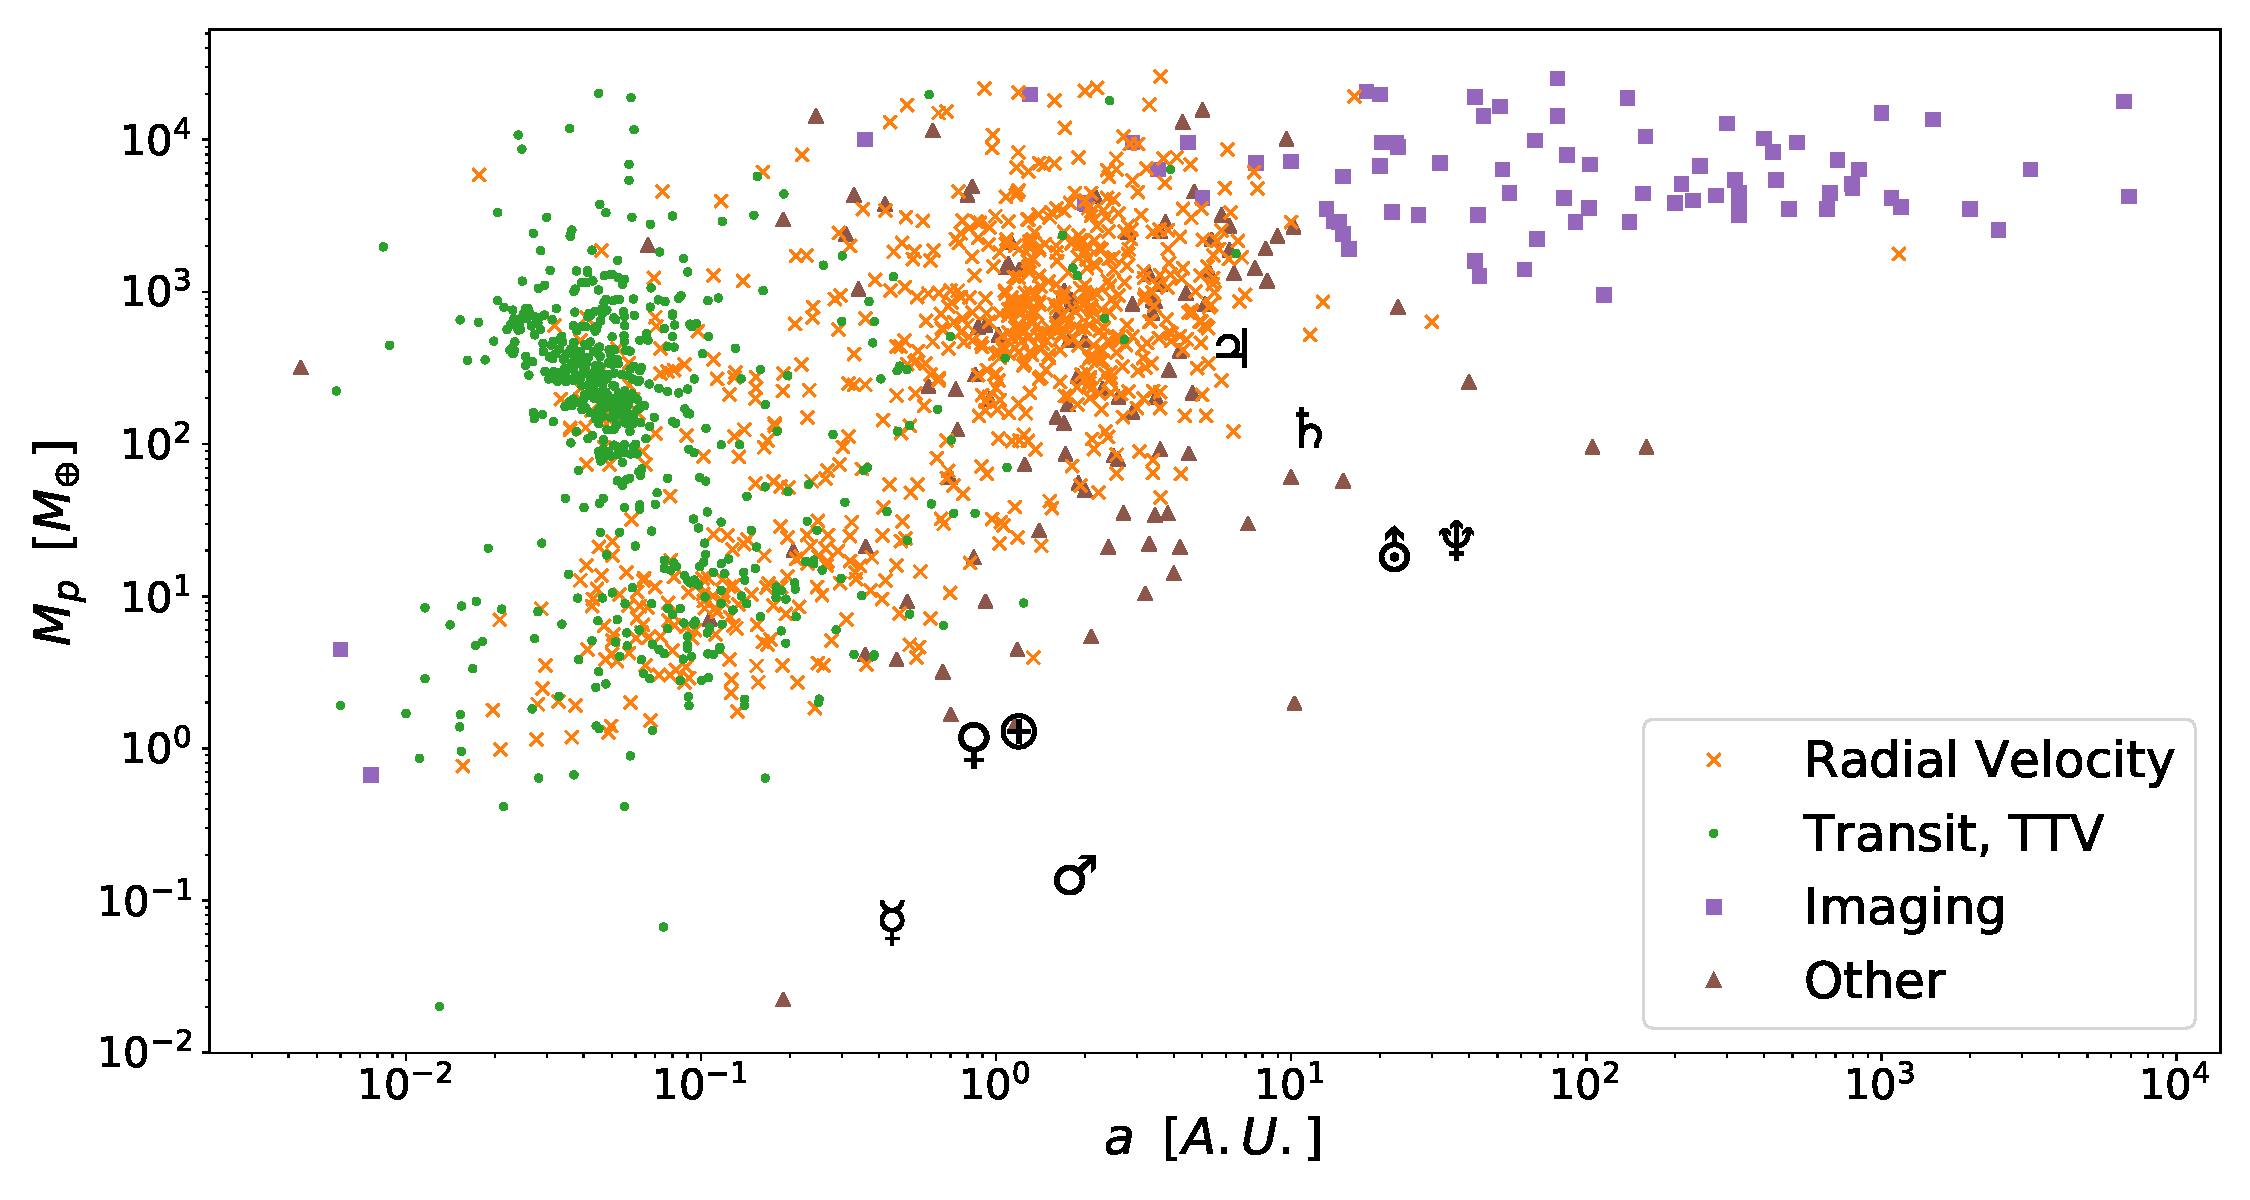
\includegraphics[width=0.7\linewidth]{./figures/introduction/exoplanetEU_a_mass.pdf}
    \caption{Distance mass diagram. 
     The symbols indicate the location of the solar system planets, $\mercury$-Mercury, $\venus$-Venus, $\earth$-Earth, $\mars$-Mars, $\jupiter$-Jupiter, $\saturn$-Saturn, $\uranus$-Uranus, $\neptune$-Neptune. Data from \href{http://ww.exoplanet.eu}{exoplanet.eu} October 2018}
    \label{fig:pltoverlayadd}
\end{figure}


Explore what these method have found with exoplanet populations.

The discovery of the hot-Jupiter class (large mass planets on close in orbits) challenged the accepted planet formation theories at the time~\citep[.e.g][]{pollack_formation_1996} in which our Solar System was thought to be typical with small rocky planets close to the Sun and large giant planets further away.



MR relation ship image arXiv:1506.05097~\citet{chen_probabilistic_2016}

\begin{figure}
    \centering
    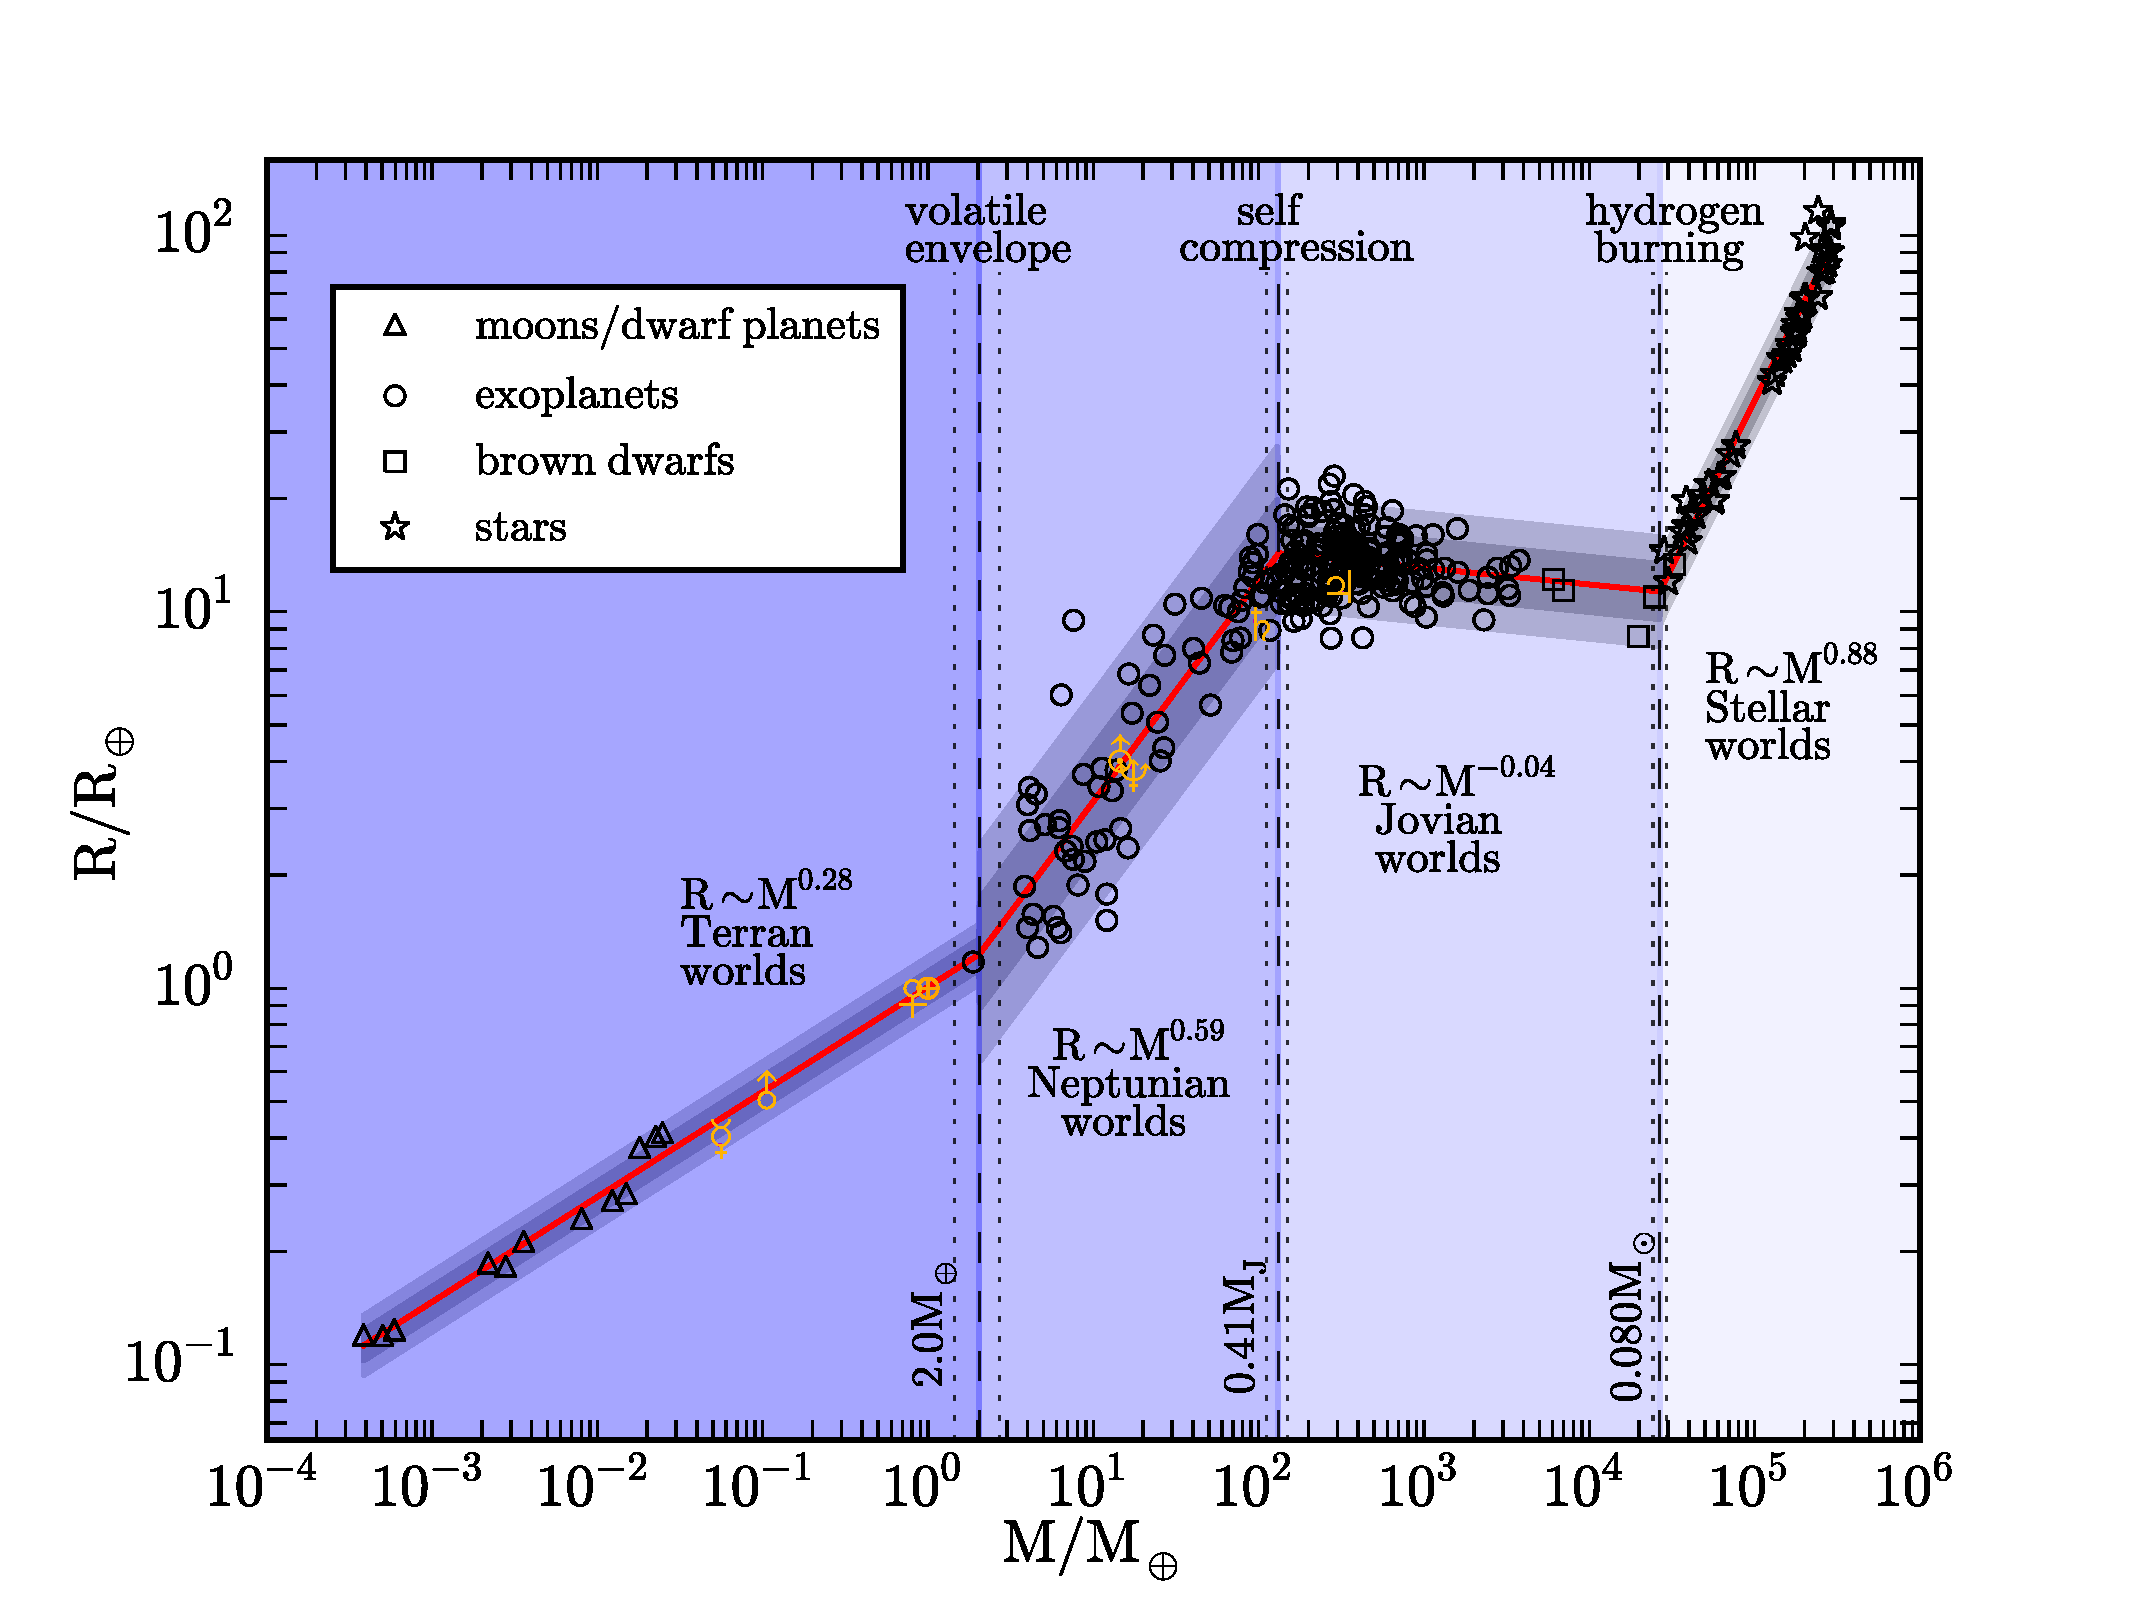
\includegraphics[width=0.4\linewidth]{./figures/introduction/mass_radius_relation.pdf}
    \caption{M-R relationship~\citet{chen_probabilistic_2016}}
    \label{fig:mass_radius_relation}
\end{figure}

Santos et al 2017 \todo{read and quote}


double peak histogram from an {RV} paper?? Faria 2018?


did they form from the molecular cloud when the star was forming or from the remnants of the disk after the star formed like exoplanets....?


\section{ conditions for life?}
habitable zone stuff
proxima b
Jorges paragraph.... 

\section{Main Section 2}


Spectral Disentangling techniques
- PSOAP
- Differencing Fruluga
- Templates?


2D-cross-correlation?   \citet{piskorz_evidence_2016} seems to have promising technique


\section{Recent detections in Companion spectra.}

Birkby


\subsection{model fitting transit stars (not actual title, more other similar methods)}
There are other situations in which to determine the presence of faint secondary spectra, such as, identifying the presence of any background or companion stars of transiting planet candidates. 
Many astronomical phenomena such as grazing eclipsing, a giant primary star eclipsed by a dwarf or a background star can produce signals indistinguishable from planetary transits. 
Efforts to characterize the false positive probability (FPP) among Kepler planet candidates is as high as $\sim35\%$~\citep{santerne_sophie_2012}.
The presence of unknown companions or background stars decreases the dimming effect from the planet transit leading to smaller planetary radius. 
Where multiple stars are present there may also be ambiguity on which star hosts the planet.
\citet{kolbl_detection_2015} developed a method for detecting the presences of faint secondary lines in optical stellar spectra by matching observations to the SpecMatch library of stellar spectra.
Identifying the spectroscopic evidence of a secondary star for 63/1\,160 California \emph{Kepler} Survey objects of Interest (KOI).


For transiting planets that presence of a background star or a companion star causes problems in characterizing the planet.
Being able to detect spectra signal of the a faint second spectra in double-lined spectroscopic binaries.
For example eclipsing binaries,
A dim binary system companion or a giant planet around a background star can mimic the transit of a small Earth-like planet on a foreground star.






\subsection{Earths atmosphere}
While the Earth's atmosphere is important for an Astronomer's lungs, it can be a nuance for their ground-based observations.
As light form astronomical sources passes through the atmosphere, its molecular components absorb some of the light, changing spectral components observed by imprinting a transmission spectrum of our atmosphere.
The \ce{H2O} absorption is a key example as it defines the photometric and spectroscopic bands in the \nir{}. \missingfigure{example to point to}.

The correction of observations from the contamination of Earth's atmosphere is a complex process.
The transmission is variable on many different time scales, the water vapour change is rapid, concentrations of atmospheric constituents, to seasonal and longer.
Such as the increase in atmospheric \ce{CO2} causing anthropamorphic climate change this requires 6\% change to \ce{CO2} line depths since 2000 Molecfit paper?
There is also variation with airmass, which depends on the observation angle in the sky and changes as targets move across the sky during the night.

other constituents, \ce{CO}, \ce{CO2}, \ce{CH4} \ldots{}, angle of observations.

An important consideration in the detecting the constituents of planetary atmospheres is the characterization and removal of Earths telluric lines.

e.g.\ 50\% error in \ce{CO2} detection on Mars atmosphere


Recently~\citet{ulmer-moll_telluric_2018} compared the telluric correction possible from three different synthetic telluric software against the standard star model.
Molecfit, a software from ESO was the most.

This is a growing field and there are other software available too\ldots{}


Water vapour content has rapid variability.
Works such as Snellen 2011, \ldots{} \ldots{} model the telluric variation during a observations to remove telluric lines and detect planetary lines.

\todo{finish this}


Telluric absorption map
\begin{figure}
    \centering
    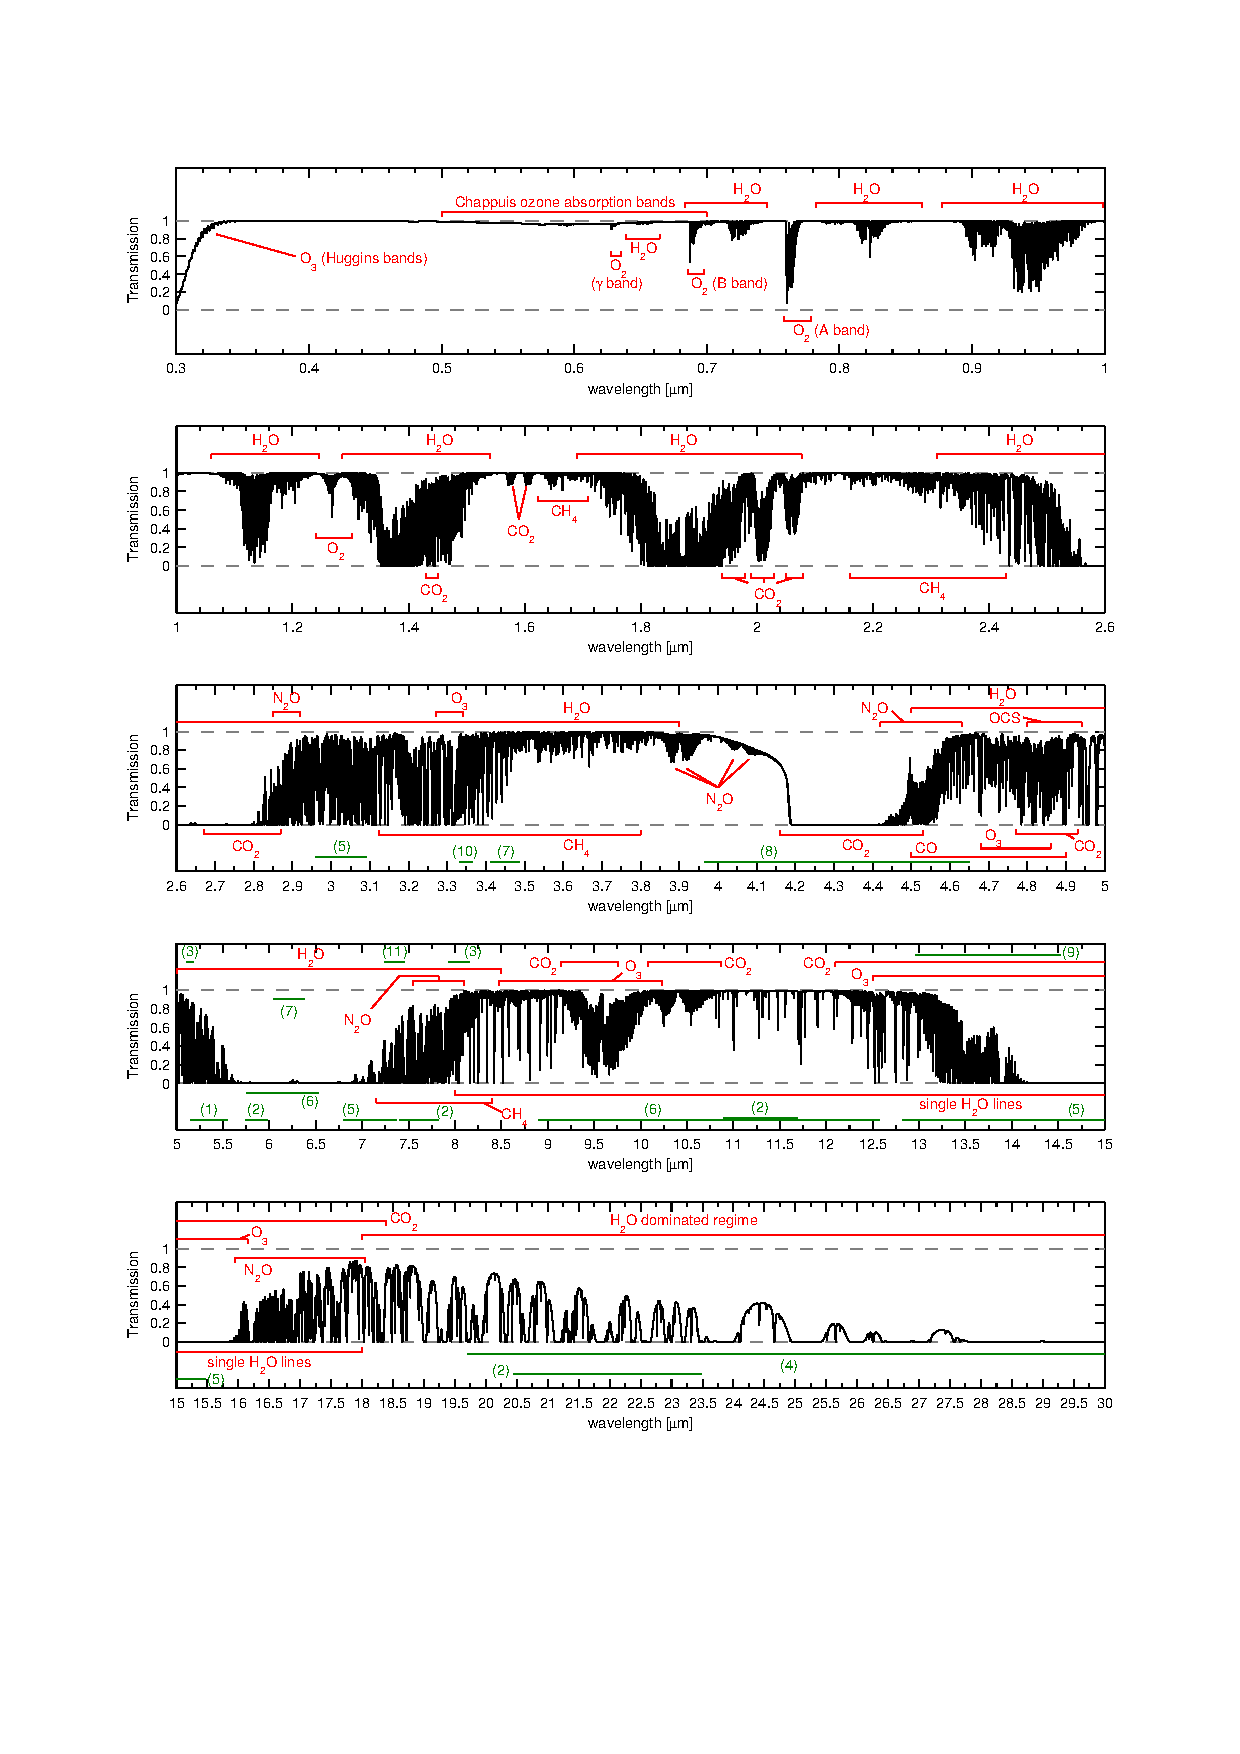
\includegraphics[width=0.9\linewidth]{figures/advanced_material/cropped_molecfit_absorbtion}
    \caption{Reproduction of Figure~1 of~\citet{smette_molecfit_2015} showing telluric absorption form 0.30 \um. Original caption:}
    \label{fig:croppedmolecfitabsorbtion}
\end{figure}
\todo{Add original caption to~\ref{fig:croppedmolecfitabsorbtion}}




\section{Paper Introduction}\label{sec:intro}
Brown dwarfs (BDs) are sub-stellar objects unable to achieve hydrogen fusion, with masses around \(13-80~\textrm{M}_{jup} \)~\citep{chabrier_theory_2000}, bridging the gap between low-mass stars and giant planets.
Without sustained fusion, brown-dwarfs cool down over time with an age-dependent cooling rate.
Therefore, there is an inherent degeneracy between the mass, age and luminosity of a given BD~\citep{burrows_nongray_1997}.
This degeneracy may be broken by observation of several parameters, for instance when a BD is in a binary system with a main sequence host star, using both the host stars age and the masses derived from the dynamical motion.

A paucity of BD companions exists in short period orbits around Sun-like stars (\(\lesssim5 \)\AU), compared to stellar or planetary companions, termed the \emph{brown dwarf desert}~\citep{halbwachs_exploring_2000, zucker_analysis_2001, sahlmann_search_2011}.
As the number of known BDs orbiting solar type stars is low, the characterization of benchmark BDs in the brown dwarf desert~\citep[e.g.][]{crepp_trends_2016} is beneficial in understanding this sub-stellar population and to help constrain formation and evolution theories~\citep{whitworth_formation_2007}.
The BD desert also provides a greater challenge as it reduces the amount of good BD candidates to study.

BDs in binary systems, unlike free-floating BDs, allow for the determination of their masses, when complemented with radial velocity ({RV}) and astrometry measurements.
The {RV} technique provides the mass lower-limit (\mtwosini{}) of binary and planetary companions, while complementary astrometry measurements can often provide mass upper-limits~\citep[e.g.][]{sahlmann_search_2011}.
Measuring or tightening the constraints of BD masses improves the understanding of mass dependence on BD formation processes.
For instance, there is growing evidence that the larger giant planets and BD companions do not follow the well known metallicity-giant planet correlation seen in main-sequence stars with planets~\citep[e.g.][]{santos_spectroscopic_2004,santos_observational_2017, maldonado_searching_2017}.
Photometry along with stellar evolution models~\citep[e.g.][]{baraffe_evolutionary_2003,allard_btsettl_2013} can also be used to estimate the mass of BD companions~\citep[e.g.][]{moutou_eccentricity_2017} if there is sufficient orbital separation, and a precise determination of the age~\citep{soderblom_ages_2010}.

Recently, there has been a renewed interest in BD candidates triggered by exoplanetary searches.
While several works found similar properties on the two populations, like a similar density~\citep{hatzes_definition_2015}, others found intriguing differences.
One of the most recent is the different host metallicity of the Brown Dwarf and giant planet populations~\citep{santos_observational_2017, schlaufman_evidence_2018}, a very strong hint of different formation mechanisms.

Spectral observations of binary systems contain the spectra of both bodies, in proportion to their flux ratio, and Doppler shifted relative to each other due to their orbital motion.
One technique to recover the spectra of the companion is secondary reconstruction through a differential spectrum~\citep{ferluga_separating_1997}.
Spectra from different phases are shifted to the host stars rest frame and subtracted to mutually cancel out the spectrum of the host star allowing the faint companion spectra to become visible.
Advances in high-resolution and near-infrared (\nir{}) capabilities should enable this technique to be applied to BDs and planet companions, in which smaller {RV} shifts can be resolved and the contrast ratio of the smaller companion is improved.

Observing in the \nir{}is specifically desirable for the cooler sub-stellar and giant planet companions as their thermal emission is stronger in the infrared compared to the optical. This improves the contrast ratio between the host star and companion, providing favourable conditions for their detection and spectral separation.
CRIRES, a high resolution \nir{} spectrograph, has made many prominent advances in recent years with the detection of atmospheric constituents, such as \(\textrm{CO} \) and \(\textrm{H}_{2}\textrm{O} \), atmospheric winds and thermal profiles, rotation and orbital motion, for both transiting and non-transiting planets~\citep[e.g.][]{snellen_orbital_2010, brogi_signature_2012, rodler_weighing_2012, dekok_detection_2013, brogi_carbon_2014, snellen_fast_2014, piskorz_evidence_2016, brogi_rotation_2016, birkby_discovery_2017}.

The higher temperature and relatively larger size of BDs compared to giant-planets makes the development of spectral recovery techniques for BD companions a logical step towards the spectroscopic detection of planetary atmospheres.
There has been the recent installation and continued development of many new high-resolution \nir{}spectrographs, such as, {CARMENES}~\citep{quirrenbach_carmenes_2014}, NIRPS~\citep{bouchy_nearinfrared_2017} or SPIRou~\citep{artigau_spirou_2014}, as well as, the {CRIRES+}~\citep{dorn_crires_2016} upgrade.
These new instruments motivate the study of \nir{}-oriented methodologies for spectral recovery, and are of high importance due to the larger planet-to-star flux ratio provided by near-IR compared to the visible.

{\rd{} The search and detection of faint secondary spectra is not only relevant to planetary atmospheres.
\citet{kolbl_detection_2015} developed a method to detect the presence of optical secondary spectra down to a flux ratio of 1\% in the hosts of \emph{Kepler} transit candidates.
The presence of which can cause ambiguities in the system configuration, and increase the uncertainty of the measured planet radius.
The characterization of the false positive probability rate for Kepler has been found to be as high as \(\sim\)35\%~\citet{santerne_sophie_2012}.}

In this paper we apply two different techniques on FGK stars with BD companions with the aim to spectroscopically detect their companions.
In \sref{sec:data} we present the observations and reduction process as well as the spectral models used in this work.
In \sref{sec:specdiff} we explain the differential spectral technique and its applicability to these observations while in \sref{sec:results} we apply companion recovery using a \textchisquared{} approach.
In \sref{sec:discussion} we discuss our results and in \sref{sec:conclusions} we present our conclusions.



brown dwarf dessert explore \citet{ranc_moa2007blg197_2015}

\section{Motivation}
